\documentclass[french, 12pt, a4paper]{article}

%%%%% PACKAGES %%%%%
\usepackage[utf8]{inputenc}
\usepackage[T1]{fontenc}
\usepackage[french]{babel}
\usepackage[margin=2cm]{geometry}
\usepackage{setspace}
\usepackage{graphicx}
\usepackage{rotating}
\usepackage{url}
\usepackage{float}
\usepackage{listings}
\usepackage{wrapfig}
\usepackage[bottom]{footmisc}
\usepackage[hidelinks]{hyperref}
\usepackage{enumitem}
\usepackage{tikz}
\def\checkmark{\tikz\fill[scale=0.4](0,.35) -- (.25,0) -- (1,.7) -- (.25,.15) -- cycle;} 
\newcommand{\subsubsubsection}[1]{\paragraph{#1}\mbox{}\\}
\setcounter{secnumdepth}{4}
\newcommand{\newpara}{\vskip 0.75cm}
\newcommand{\newparasm}{\vskip 0.2cm}

\begin{document}
\singlespacing

%%%%% PAGE DE GARDE %%%%%

\begin{titlepage}
\begin{center}


\includegraphics[width=15cm]{img/ephec.jpg}~\\
\textsc{Avenue du Ciseau, 15 \\ 1348 Ottignies-Louvain-la-Neuve} \\[1.5cm]

{\huge \bfseries \begin{spacing}{1.25}
  Application web \\ 
  de gestion de la supply-chain \\
  pour la société SLG Classic Cars \\
  \LARGE(restauration de véhicules anciens)
  \\[2cm]
  \end{spacing} 
} 

{\large 
  Travail de fin d'études présenté en vue de l'obtention du diplôme de bachelier
  en Informatique et Systèmes Orientation Technologie de l'Informatique
  \\[2cm]
}

{\LARGE 
  MICHOTTE Martin
}

\vspace*{\fill}
\textsc{\large Rapporteur: M-N. VROMAN}
\hfill
\textsc{\large Année académique 2020-2021}

\end{center}
\end{titlepage}

%%%%% REMERCIEMENTS %%%%%
\onehalfspacing
\setcounter{page}{0}
\addtocontents{toc}{\protect\setcounter{tocdepth}{0}}
\section*{Remerciements}

%%%%% TOC %%%%%
\singlespacing
\newpage
\addtocontents{toc}{\protect\setcounter{tocdepth}{4}}
\renewcommand{\contentsname}{Table des matières}
\tableofcontents

%%%%% CONTENU %%%%%
\onehalfspacing

\newpage
\section{Introduction}
\subsection{Contexte}
\subsubsection{Client}

Le client, SLG Classic Cars, est une petite société familiale de restauration et entretien de voitures anciennes. Elle a été initialement fondée en 1976 et a été reprise par les fils en 2015. Ils sont désormais réputé dans leurs domaines et ne cessent de développer leurs activités. La société est basée sur deux sites, un atelier mécanique à Bierwart ainsi qu'un atelier carrosserie à Hingeon. 

\newpara

Dans le cadre de leurs activités, la societé a besoin d'un SI\footnote{\textit{"Le système d’information (SI) est un élément central d’une entreprise ou d’une organisation. Il permet aux différents acteurs de véhiculer des informations et de communiquer grâce à un ensemble de ressources matérielles, humaines et logicielles. Un SI permet de créer, collecter, stocker, traiter, modifier des informations sous divers formats."}\cite{SI}} permettant de gérer de manière efficace les informations relatives aux:
\begin{itemize}
  \item clients 
  \item fournisseurs
  \item véhicules
  \item stock
  \item commandes
  \item devis
  \item factures
  \item fiches de Travail
  \item ...
\end{itemize}

\subsubsection{Solution existante} 

Jusqu'à présent la société utilise une combinaison de deux logiciels:
\begin{description}
  \item[GAD-Garag] : \textit{"Le logiciel garage GAD Garage est un logiciel garage professionnel de gestion commerciale pour la réparation de véhicule , GAD Garage est un logiciel Garage pour Auto , moto et la vente de pièces détachées automobiles (semi-grossiste)."}\cite{GAD}
  \item[SLG-order-manager] : Logiciel propriétaire permettant de générer et réceptionner des commandes. Ce logiciel intéragit directement avec GAD-Garage et permet de simplifier l'encodage des informations relatives au stock. 
\end{description}

\newpara

En raison de divers problèmes liés au logiciel GAD-Garage et un manque de maintenance de celui-ci, la société souhaite développer une nouvelle solution informatique spécialement adaptée à leur façon de travailler et à leurs besoins cités ci-avant. Cette solution doit être conçue de façon à pouvoir être adaptée au fil des années en fonction des nouveaux besoins du client.

\subsection{Objectifs}

Au vue de l'envergure du projet et un temps relativement limité quant à la réalisation de ce travail de fin d'études, le client et moi-même avons décidé de définir des objectifs à court et long termes. Les objectifs à court termes sont prioritaires et sont ceux sur lesquels je travaillerai dans le cadre de ce travail de fin d'études. Si le résultat est concluant le projet sera étendu au delà du cadre scolaire et les objectifs à plus long termes seront réalisé. 

\newpara

Bien que les objectifs à long terme soient moins importants, ils ne sont pas indispensables pour autant. Dès lors, durant toute la durée de développement de ce projet, le client continuera d'utiliser ses solutions actuelles. 

\subsubsection{Court terme}

\begin{itemize}
  \item gestion des clients 
  \item gestion des fournisseurs
  \item gestion du stock
  \item gestion de la main d'oeuvre
  \item gestion des commandes 
  \item design "user-friendly"
  \item déploiement
\end{itemize}

\newpara

Ces différents objectifs sont assez vaste et cachent une multitude d'objectifs secondaires tel que la gestion des droits aux ressources, la gestion de conflit d'encodage\footnote{Gérer la possibilité que deux utilisateurs distincte modifier simultanément une même donnée.} et bien d'autres.  

\subsubsection{Long terme}

\begin{itemize}
  \item les autres fonctionnalités (voitures, facturation, ...)
  \item gestion avancée des utilisateurs de la web-App
\end{itemize}

\newpage
\section{Recueil d'information et Analyse}

Après avoir défini, avec le client, les grandes lignes du projet il a fallu définir et détailler de manière approfondie toutes les fonctionnalités. Pour ce faire, j'ai décidé de procéder en plusieurs étapes. 

\newpara

\textbf{Premièrement}, plusieurs réunions avec le client ont permis de dégrossir l'ensemble des fonctionnalités. Ainsi, chaque grosse fonctionnalité a été découpée en plus petites, a été détaillée en texte clair et a été contextualisée par rapport à l'ensemble du projet. 
Cette étape fut très importante car elle a permis de concrétiser les besoin du client et de mettre en avant les potentielles difficultés. 

\newpara

\textbf{Dans un second temps}, sur base de l'étape précédente, j'ai transformé le texte claire de chaque fonctionnalité en "user story"\footnote{Une "user story" est, dans le domaine du développement de logiciels, une description simple et structurée d'une fonctionnalité à développer.} Les "user stories" permettent de structurer l'ensemble des fonctionnalité en un format bien défini. Plus d'information quand à la réalisation de celles-ci se trouvent dans le sous-chapitre "User-stories" ci-après. 

\newpara

\textbf{Pour finir}, j'ai analyser et défini avec le client les besoins plus techniques tel que par exemple: 
\begin{itemize}
  \item les liens inter-fonctionnalité
  \item les données à devoir stocker 
  \item les liens entre les différentes données
  \item les implications comptable (au niveau du stock et de la facturation)
  \item une estimation de la quantité de donnée à stocker
  \item les roles des différents utilisateurs
\end{itemize}

\newpage

\subsection{User-stories}

Comme expliqué précédemment, chaque fonctionnalité à été détaillée sous forme d'une "user story" (US). Dans un but organisationnel, j'ai décidé de grouper chaque US par grande fonctionnalité. Qu'entend-t-on par grande fonctionnalité? Dans le cadre de ce projet, une grande fonctionnalité est un élément fictif faisant référence à l'ensemble des informations et manipulations relatives à un objet du système d'information. A titre d'exemple: la grande fonctionnalité "\textbf{Stock}" regroupe l'ensemble des fonctionnalités permettant de définir la façon dont un utilisateur va pouvoir consulter la quantité restante d'un produit, l'historique d'achat ou de vente d'un produit, la valeur cumulée de tous les produits, ajouter un nouveau produit, etc. 

\newpara

Afin de pouvoir facilement maintenir la multitude d'US, j'ai défini un structure type comportant les éléments suivants :
\begin{enumerate}
  \item Code unique + Titre
  \item Description (du type: \textit{"En tant que X j'aimers Y afin de Z"})
  \item Préconditions
  \item Explication détaillée avec éventuellement des mockups\footnote{\textit{"En informatique, le terme mock-up (qui vient du même mot anglais qui signifie une maquette à l'échelle 1:1) désigne un prototype d'interface utilisateur."}\cite{Mock}}
  \item Critères de validation
\end{enumerate}

\newpage

\subsubsection{Exemple}

\begin{figure}[H]
  \centering
  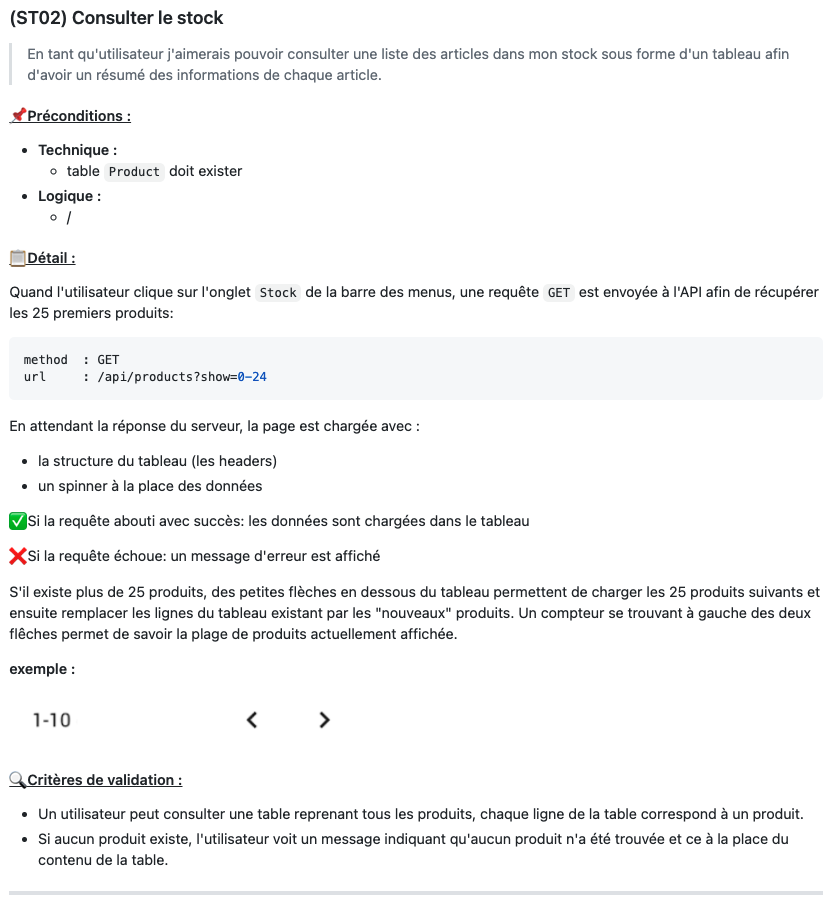
\includegraphics[width=\textwidth]{img/exemple_us.png}
  \caption{Exemple de "user story"}
\end{figure}

L'ensemble des US peuvent-être consultées dans la wiki de la page Github\footnote{\url {https://github.com/MMichotte/SLG_APP/wiki/US_0_home}} de ce projet. 
Notons que toutes les fonctionnalités n'ont pas été transformées en US. J'ai décidé de travailler selon les méthodes de développement "agiles" qui préconisent de ne pas réaliser l'entièreté de l'analyse si cela n'est pas nécessaire au développement. Ma méthodologie de travail est décrite dans un chapitre ultérieur. 

\newpage

\subsubsection{Automatisation Trello}
Une fois une US écrite, je la re-transcrivait sous forme de carte "Trello"\footnote{Trello est un programme des gestion de taches permettant de créer différentes listes et cartes fin d'organiser le travail. Pour plus d'informations voir : \url{https://trello.com}} afin de pouvoir utiliser celle-ci comme base de travail lors de l'implémentation de la fonctionnalité. Cette opération étant fastidieuse et rébarbative, j'ai décidé de développer une petite application en ligne de commande me permettant d'automatiquement générer mes cartes Trello sur base de mes US écrites dans la wiki du Github du projet. 

\newpara

J'ai conçu cette application avec comme objects: 
\begin{enumerate}
  \item imposer une structure d'US
  \item utilisation simple
  \item possibilité d'intégration dans une pipeline de déploiement continu\footnote{Une pipeline de déploiement continu est un ensemble d'actions permettant d'automatiser le déploiement du code depuis un environnement de développer vers un environnement de production. Pour de plus amples informations voir: \url{https://www.redhat.com/fr/topics/devops/what-is-ci-cd}}
  \item ne doit pas avoir d'impact visuel sur les US dans le wiki de github
  \item open-source
\end{enumerate}

\newpara

Bien que la conception de cette application m'ai pris un certain temps, cela est dérisoire par rapport au gain de temps que j'ai pu en tirer. Les fonctionnalités proposée par cette application sont néanmoins encore limités mais le projet étant open-source, tout le monde peut y contribuer. 

\newpara

Une explication plus détaillé n'ayant pas sa place dans ce rapport, elle est disponible sur le Github de ce mini-projet: \url{https://github.com/MMichotte/US-to-TrelloCard}.


\subsection{Base de donnée}
Un bon système d'information repose en grande partie sur la qualité de la base de donnée.  
//TODO 

\begin{sidewaysfigure}
  \centering
  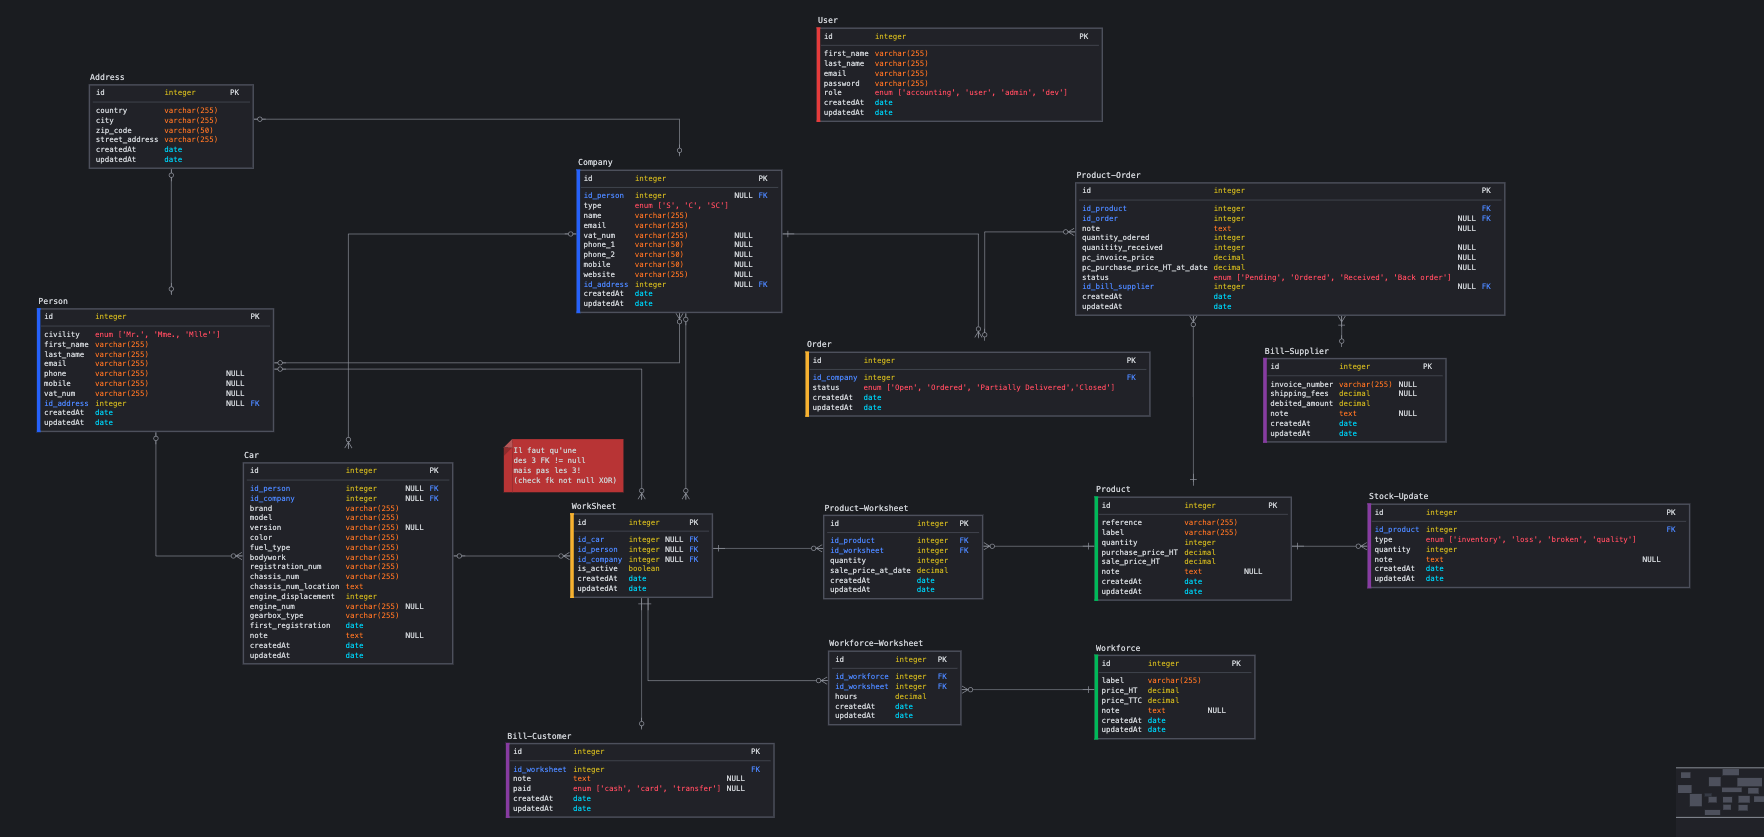
\includegraphics[width=\textwidth]{img/DB-schema.png}
  \caption{Schéma de base de donnée}
\end{sidewaysfigure}

\newpage
\section{Méthodologie}
\subsection{Agile}

Comme brièvement abordé précédemment, vu la l'envergure et la complexité du projet, j'ai décidé de travailler de manière "agile". Mais qu'est-ce que "l'agilité" dans le monde du développement informatique? \textit{"En ingénierie logicielle, les pratiques agiles mettent en avant la collaboration entre des équipes auto-organisées et pluridisciplinaires et leurs clients1. Elles s'appuient sur l'utilisation d'un cadre méthodologique léger mais suffisant centré sur l'humain et la communication2. Elles préconisent une planification adaptative, un développement évolutif, une livraison précoce et une amélioration continue, et elles encouragent des réponses flexibles au changement"\cite{Agile}}.

\newpara

Concrètement, dans le cadre de ce projet, cela à impliqué que j'ai travaillé de manière incrémentale comme l'illustre la \textit{figure \ref{agile}} ci-dessous. 
\begin{figure}[H]
  \centering
  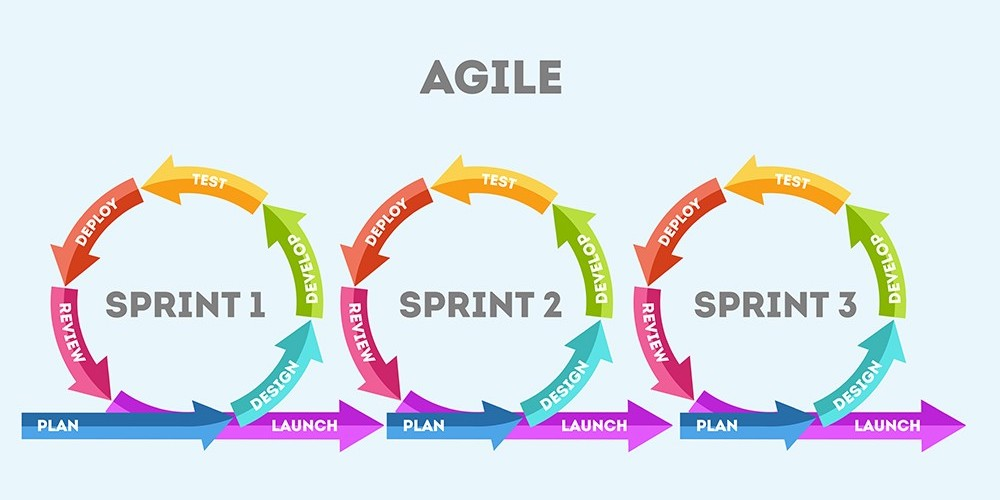
\includegraphics[width=0.75\linewidth]{img/agile.jpeg}
  \caption{ \textit{Les raisons pour utiliser les méthodes Agile en entreprise} de 300\_librarians}
  \label{agile}
\end{figure}
Chaque fonctionnalité de ce projet peut être representée par un "sprint". En d'autres termes j'ai, pour chaque fonctionnalité: 
\begin{enumerate}
  \item détaillé sous forme d'une US (PLAN + DESIGN) 
  \item implémenté (DEVELOP)
  \item testé par le biais de tests automatisé ou manuellement (TEST)
  \item déployé l'ensemble en production (DEPLOY)
  \item demandé un feedback au client (REVIEW)
  \item adapté la fonctionnalité en fonction du feedback 
\end{enumerate} 

\newpara

Cette Méthodologie a été très efficace et a permis une bonne collaboration avec le client. 

\subsection{Choix des technologies}
\subsubsection{Backend}
\begin{figure}[H]
  \begin{minipage}{.3\textwidth}
    
\includegraphics[width=0.75\linewidth]{img/tech/NestJs.png} 
  \end{minipage}
  \begin{minipage}{.7\textwidth}
    \begin{description}
      \item[Framework]: NestJs
      \item[Language]: TypeScript
      \item[Runtime environnement]: NodeJs  
      \item[ORM]: TypeOrm 
    \end{description}
    Tout d'abord, vu l'envergure du projet, il me paraissait important de veiller à une bonne structure et de garder en tête la maintenance du projet au fil du temps. Dans ces circonstances, il est important d'utiliser un framework. Quant au choix du framework, dans un premier temps mon choix s'est porté sur la suite NodeJs-ExpressJs. Ce choix était initialement justifié par le fait que j'avais déjà travailler avec ceux-ci. Après quelques semaines de développement, je me suis rendu compte que je préférait nettement utiliser le TypeScript pour un projet d'une tel envergure. J'ai des lors décidé de changer de framework et ai migré mon application NodeJs-Express vers du NestJs. Le NestJs utilise du Typescript et permet de bien structurer son code comme au frontend avec Angular. (voir ci-après)
  \end{minipage}
\end{figure}

\subsubsection{Frontend}
\begin{figure}[H]
  \begin{minipage}{.3\textwidth}
    
\includegraphics[width=0.75\linewidth]{img/tech/Angular.png}
  \end{minipage}
  \begin{minipage}{.7\textwidth}
    \begin{description}
      \item[Framework]: Angular
      \item[Languages]: \begin{itemize}
        \item TypeScript
        \item HTML
        \item SCSS
      \end{itemize} 
    \end{description}
    Tout comme pour le backend, il est évident que l'utilisation d'un framework est indispensable. Le choix du framework s'est fait sur base de mon expérience personnelle. En effet, durant mes années d'études, j'ai eu l'occasion d'utiliser différent frameworks frontend tel que React, Vue et Angular. J'ai particulièrement bien aimé travailler avec ce dernier car il impose une certaine rigueur tout en restant relativement simple d'utilisation.
  \end{minipage}
\end{figure}

\newpage

\subsubsection{Base de donnée}

\begin{figure}[H]
  \begin{minipage}{.3\textwidth}
    
\includegraphics[width=0.75\linewidth]{img/tech/PostgreSql.png} 
  \end{minipage} 
  \begin{minipage}{.7\textwidth}
    Le choix de la base de données a été motivé par trois critères :
    \begin{enumerate}
      \item \textbf{SQL}: Comme expliqué lors de l'analyse des besoins du client dans la section "Base de donnée", vu le grand nombre de relations entre les différentes données, une base de données SQL est primordiale pour la bonne organisation du système d'information.
      \item \textbf{Notoriété}: PostgreSQL est fortement utilisé dans le milieu proféssionnel ce qui lui oblige d'être mis à jour régulièrement et ce tant au niveau sécurité que en ajout de fonctionnalités. C'est donc une base de données fiable, utilisable à long terme et maîtrisée par de nombreux développeurs.
      \item \textbf{Expérience}: Bien que toutes les bases de données SQL se ressemble, le fait d'avoir déjà manipuler et de s'être familiariser avec PostgreSql m'offre un gain de temps considérable.
    \end{enumerate}
  \end{minipage} 
\end{figure}

\subsubsection{Autre}

\subsubsubsection{API}

Afin de tester les différents endpoints API de l'application, j'ai décidé d'utiliser \textbf{Insomnia}\footnote{\url{https://insomnia.rest}}. Insomnia permet non seulement de tester mon API en temps réel mais permet aussi d'écrire la documentation. Je n'utiliserai néanmoins pas cette dernière fonctionnalité étant donnée que le framework backend (NestJs) que j'utilise me permet de générer automatiquement et facilement une documentation API.

\newpara

Une API sans documentation est pratiquement inutilisable. Il existe un grand nombre de technologies pour écrire de la documentation API. Afin de centraliser un maximum d'éléments, j'ai décidé d'utiliser un plugin pour NestJs. Ce plugin (swagger swagger-ui-express\footnote{\url{https://docs.nestjs.com/openapi/introduction}}) me permet de générer automatiquement la documentation de mes endpoints sur base de quelques décorateurs\footnote{Code non-essentiel au fonctionnement de l'application mais permettant d'écrire des annotations} ajouté dans le code. En plus de cela, il me permet de de déployer cette documentation directement avec l'application. Celle-ci est dès lors consultable ici:\\\url{https://app.slgcars.be/api-docs/}.

\newpage

\subsubsubsection{Linter}

Il est "facile" d'écrire du code mais beaucoup plus compliqué de le rendre cohérent, lisible et portable. Afin de palier à ces problèmes un linter est indispensable. Étant donnée que je travaille principalement avec du JS et du TS, j'ai opté pour ESLint. Ce linter est 100\% configurable pour chaque projet et me permet de garantir, dans l'éventualité où dans le future un autre développeur venait à contribuer au projet, la cohérence de nommage des variables, la configuration de l'IDE et bien d'autre choses. Pour ce qui est du HTML et SCSS un linter est inclus dans le framework Angular.

\subsection{Outils}


\newpage
\section{Développement}

Bien que le développement à proprement parler ait constitué la majeure partie de ce projet, expliquer l'intégralité des fonctionnalités n'a pas sa place dans le cadre de ce rapport. Je tiens cependant à partager un exemple d'une analyse logique d'une fonctionnalité qui, à mes yeux, représente bien la complexité de ce projet (voir \textit{\ref{exemple_dev}}). 

\newpara

Le développement a été divisé en quatre grandes phases :
\begin{enumerate}
  \item \textbf{Mise en place de la structure du projet}: \\ Cette phase a consisté à initialiser les différents modules du projet (backend, frontend, ...) ainsi qu'a choisir une structure de dossier appropriée. 
  \item\textbf{Mise en place des outils facilitant le productivité}: \\ Afin de simplifier le travail et/ou de ne pas devoir exécuter des tâches répétitives, j'ai utilisé plusieurs outils tel qu'un linter\footnote{Un linter est un outil d'analyse statique de code permettant d'uniformiser le style du code et de déceler des potentiels erreurs.} ou des extensions de mon IDE me proposant de l'autocomplétion avancée. Ce sont donc une série d'outils non-indispensables mais fort utiles.
  \item \textbf{Implémentation des US}
  \item \textbf{Refactoring}: \\ Cette phase n'est pas une phase en tant que telle. En effet, tout au long du projet, j'ai refactorisé le code que ce soit au niveau de la structure ou de la logique. 
\end{enumerate}

\subsection{Exemple concret}
\label{exemple_dev}
\textbf{Contexte}: Dans le cadre de la US \textit{"CO07 - Réceptionner une commande"}, une multitude de cas sont à étudier. En voici l'analyse: 

\newpara

Pour chaque produit réceptionné:
\begin{enumerate}

  \item \textbf{Le produit a été reçu avec: quantité reçue == quantité commandée}
  \begin{enumerate}
    \item mise à jour de l'information du produit
    \item le statut du produit passe à "RECEIVED"
  \end{enumerate}

  \newpara
  \item \textbf{Le produit a été reçu avec: quantité reçue < quantité commandée}
  \begin{enumerate}
    \item Le produit est affiché avec deux status: "RECEIVED" et "BO"\footnote{Back Order}. La quantité manquante est affichée dans le statut "BO".
    \newpage
    \item Lors de la sauvegarde de la facture:
    \begin{enumerate}
      \item un nouveau produit reprenant les mêmes informations que le produit d'origine est ajouté à la commande courante. La quantité commandée de ce nouveau produit est égale à la quantité manquante définie précédemment. Le statut de ce produit est "BO".
      \item le statut produit d'origine passe à "RECEIVED".
    \end{enumerate}
  \end{enumerate}
  
  \newpara
  \item \textbf{Le produit a été reçu avec: quantité reçue > quantité commandée}
  \begin{enumerate}
    \item Le système cherche tous les produits équivalents à celui-ci venant du même fournisseur et dont le statut est "BO". 
    \begin{itemize}
      \item \textbf{le système trouve un produit}: 
      \begin{enumerate}
        \item Récupération de la commande concernée par le produit trouvé
        \item Traitement de ce produit comme s'il faisait partie de la commande actuelle (il passe par les mêmes étapes décrites dans ici)
      \end{enumerate}
      \item \textbf{le système ne trouve pas de produit}: On continue la procédure ci-dessous
    \end{itemize}
    \item mise à jour de l'information du produit
    \item le statut du produit passe à "RECEIVED"
  \end{enumerate}
  
  \newpara
  \item \textbf{Le produit n'a pas été reçu}
  \begin{enumerate}
    \item le statut du produit passe à "BO"
  \end{enumerate}

  \newpara
  \item \textbf{Le produit ne faisait pas partie de la commande concernée}
  \begin{enumerate}
    \item l'utilisateur a la possibilité d'ajouter un produit non-présent dans la commande à l'aide d'un bouton.
    \item (ajout du produit dans la commande, voir US CO03)
    \item retour à l'étape n° 3
  \end{enumerate}

\end{enumerate}

\newpara

La réception d'une commande génère une facture. Cette facture a une valeur comptable et doit donc être correcte. En plus de la création d'une facture, la réception d'une commande met à jour le stock. Le stock étant d'une grande importance financière et commerciale, celui-ci doit également être le plus exact possible. Dans ces circonstances, il était impératif que toutes les actions exécutées sur tous les produits d'une commande soient bloquants en cas d'erreur. Dès lors, j'ai utilisé un système de transaction afin de garantir l'intégrité des données. Soit l'intégralité des données sont correctes et cohérentes et sont alors ajoutées en base de données, soit il y a une erreur et l'entièreté de l'action est annulée, aucun changement n'a lieu dans la base de données. 

\newpage

\subsection{Récapitulatif des fonctionnalités/US implémentées}
L'ensemble des fonctionnalités prévues dans les objectifs à "court terme" ont été réalisées. Voici un récapitulatif non-détaillé des US implémentées:  

\newpara
\textbf{Général}
\begin{itemize}
  \item \checkmark G01 - Connexion utilisateur
\end{itemize}

\newpara
\textbf{Stock}
\begin{itemize}
  \item \checkmark ST01 - Onglet Stock
  \item \checkmark ST02 - Consulter le stock
  \item \checkmark ST03 - Ajouter nouvel article dans le stock
  \item \checkmark ST07 - Rechercher un article
  \item \checkmark ST09 - Supprimer un article
  \item \checkmark ST04 - Consulter/modifier le détail d'un article
  \item \checkmark ST06 - Consulter récapitulatif entrée/sortie d'un article
\end{itemize}

\newpara
\textbf{Main d'oeuvre}
\begin{itemize}
  \item \checkmark MO01 - Onglet Main d'oeuvre
  \item \checkmark MO02 - Consulter la liste des main d'oeuvre
  \item \checkmark MO03 - Ajouter un nouveau tarif de main d'oeuvre
  \item \checkmark MO05 - Rechercher une main d'oeuvre
  \item \checkmark MO06 - Supprimer une main d'oeuvre
  \item \checkmark MO04 - Consulter/Modifier le détail d'une main d'oeuvre
\end{itemize}

\newpara
\textbf{Client}
\begin{itemize}
  \item \checkmark CL01 - Onglet Clients
  \item \checkmark CL02 - Consulter liste clients
  \item \checkmark CL03 - Ajout nouveau client
  \item \checkmark CL09 - Rechercher un client 
  \item \checkmark CL10 - Supprimer un client
  \item \checkmark CL04 - Consulter/modifier détail d'un client
\end{itemize}

\newpage

\textbf{fournisseur}
\begin{itemize}
  \item \checkmark FO01 - Onglet Fournisseurs
  \item \checkmark FO02 - Consulter liste des fournisseurs
  \item \checkmark FO03 - Ajouter nouveau fournisseur
  \item \checkmark FO04 - Consulter/Modifier le détail d'un fournisseur
  \item \checkmark FO06 - Rechercher un fournisseur
  \item \checkmark FO07 - Supprimer un fournisseur
\end{itemize}

\newpara
\textbf{Commandes}
\begin{itemize}
  \item \checkmark CO01 - Onglet Commandes
  \item \checkmark CO02 - Consulter la liste des commandes
  \item \checkmark CO03 - Créer une nouvelle commande
  \item \checkmark CO04 - Consulter le détail d'une commande
  \item \checkmark CO05 - Rechercher une commande
  \item \checkmark CO06 - Supprimer une commande
  \item \checkmark CO07 - Réceptionner une commande
\end{itemize}

\newpara
\textbf{Factures}
\begin{itemize}
  \item \checkmark FA01 - Onglet Factures
\end{itemize}

\newpara
Une série de captures d'écrans de l'interface utilisateur peut être consultée en annexe de ce document.

\newpage
\section{Sécurité}

\subsection{Contrôle d'accès}
Cette application web est destinée à être utilisée par plusieurs personnes avec des rôles différents au sein de la société. Chaque rôle n'a pas les mêmes droit quant à la consultation ou manipulation des données de l'application. On peut ainsi distinguer cinq catégories d'utilisateurs: 
\begin{enumerate}
  \item \textbf{Inconnu}: utilisateur non-authentifié. Celui-ci n'a aucun droit sur les données et peut uniquement accèder à la page de connexion de l'application. 
  \item \textbf{Comptabilité}: 
  \begin{itemize}
    \item a tous les droits de l'inconnu
    \item peut uniquement consulter l'ensemble des données 
    \item peut générer des pdf (factures, commandes, ...)
  \end{itemize}
  \item \textbf{Atelier}: 
  \begin{itemize}
    \item a tous les droits de la comptabilité
    \item peut créer/modifier une fiche de Travail
    \item peut créer/modifier une commande
  \end{itemize}
  \item \textbf{Administration}: 
  \begin{itemize}
    \item peut tout faire hormis supprimer les utilisateurs de type "Développeur"
  \end{itemize}
  \item \textbf{Développeur}: 
  \begin{itemize}
    \item peut tout faire et a accès aux logs et métriques
  \end{itemize}
\end{enumerate}

\newpara

Afin d'authentifier un utilisateur et donc de lui donner certain droits ou non, l'application utilise des JSON Web Tokens (JWT)\footnote{Comment cela fonctionne-t-il? Explication en vidéo: \url{https://www.youtube.com/watch?v=7Q17ubqLfaM}}. Les tokens sont générer lors de chaque nouvelle connexion réussie et sont valide pendant 48h. Toute action effectuée à l'aide d'un token non-valide déconnecte automatiquement l'utilisateur et le re-dirige vers la page de connexion. 

\newpage

\subsection{Hachage et Chiffrement}

Avant toute choses il me semble bon de rappeler la différence entre le \textbf{hachage} et le \textbf{chiffrement}: 
\begin{itemize}
  \item \textbf{hachager}: \\ Utilisation d'un algorythme de hachage uni-directionnel afin de transformer les données de manière irréversible et de longueur fixe. Il est donc possible de comparé deux hash.
  \item \textbf{chiffrer}: \\ Encoder des données afin qu'uniquement la personne ayant la clé de déchiffrement puisse les déchiffrer. Cette action est donc réversible.
\end{itemize}

\subsubsection{Données enregistrées}
Toute donnée susceptible d'être un risque pour l'intégrité et la protection de l'application ou des autres données est stockée sous forme de hash (et non en clair\footnote{lisible et comprehensible par quiconque}) dans la base de données (par exemple les mots de passes des utilisateurs). 

\newpara

Afin de hasher ces données, j'ai utilisé la librairie "bcrypt". La librairie "bcrypt" est une des librairies de hashage les plus réputées. Elle permet d'incorporer un sel (salt)\footnote{\textit{"Le salage, est une méthode permettant de renforcer la sécurité des informations qui sont destinées à être hachées (par exemple des mots de passe) en y ajoutant une donnée supplémentaire afin d’empêcher que deux informations identiques conduisent à la même empreinte (la résultante d’une fonction de hachage)"}\cite{Salt}} afin de se protéger contre les attaques par table de correspondance (rainbow table)\footnote{Attaque consistant à comparer un hash à un table reprenant un grand nombre de paires de text clair et le hash correspondant.}. De plus elle est facilement paramétrable permettant ainsi d'augmenter la complexité de l'algorithme utilisé afin de palier aux attaques par force brute\footnote{Attaque consistant à essayer un grand nombre de donnés générées automatiquement en espérant trouver la bonne.} utilisant des machines à puissances de calcule importante. 

\subsubsection{HTTPS}
Stocker les données à risque de manière chiffrée dans la base de données est une chose, cependant, avant que les données n'arrivent jusque là elles sont potentiellement envoyées en clair sur le réseau (internet). Afin d'éviter cela, je n'autorise que les connexion HTTPS et redirige les connexions HTTP vers le HTTPS. Ceci permet de garantir que l'entièreté des données envoyées sont chiffrées et dès lors beaucoup moins vulnérables aux attaques de type "Man In The Middle" (MITM).

\newpage

\subsection{HTTP Headers}

Les headers HTTP permettent de sécuriser un site-web contre la plupart des attaques les plus répendues et ce de manière relativement simple. Voici en résumé les principaux headers que j'ai configuré:

\begin{itemize}
  \item \textbf{Strict-Transport-Policy (STP)}: \\ Header permettant d'indiquer au navigateur que le site-web ne peut être accèder qu'en utilisant HTTPS au lieu de HTTP. \\
  
  \item \textbf{Content-Security-Policy (CSP)}: \\ \textit{"L'en-tête de réponse HTTP Content-Security-Policy permet aux administrateurs d'un site web de contrôler les ressources que l'agent utilisateur est autorisé à charger pour une page donnée. Bien qu'il y ait quelques exceptions, ces règles impliquent la plupart du temps de définir les origines du serveur et les points d'accès pour les scripts. Cet en-tête aide à se protéger contre les attaques de cross-site scripting."}\cite{CSP} \\

  \item \textbf{X-Frame-Options}: \\ \textit{"L'en-tête de réponse HTTP X-Frame-Options peut être utilisé afin d'indiquer si un navigateur devrait être autorisé à afficher une page au sein d'un élément <frame>, <iframe>, <embed> ou <object>. Les sites peuvent utiliser cet en-tête afin d'éviter les attaques de clickjacking pour s'assurer que leur contenu ne soit pas embarqués dans d'autres sites."}\cite{X-Frame} \\

  \item \textbf{X-Content-Type-Policy}: \\ \textit{"L'entête X-Content-Type-Options est un marqueur utilisé par le serveur pour indiquer que les types MIME annoncés dans les en-têtes Content-Type ne doivent pas être modifiés ou et suivis. Cela permet de se détacher du sniffing de type MIME, ou, en d'autres termes, c'est une façon de dire que les webmasters savaient ce qu'ils faisaient."}\cite{X-Content}
\end{itemize}

\newpara

Après avoir configuré ces différents headers, j'ai testé le bon fonctionnement de ceux-ci en lançant une analyse en ligne. Comme le montre la \textit{figure \ref{Headers}} l'ensemble des headers ont bien été configurés et protègent désormais le site-web. 

\begin{figure}[H]
  \centering
  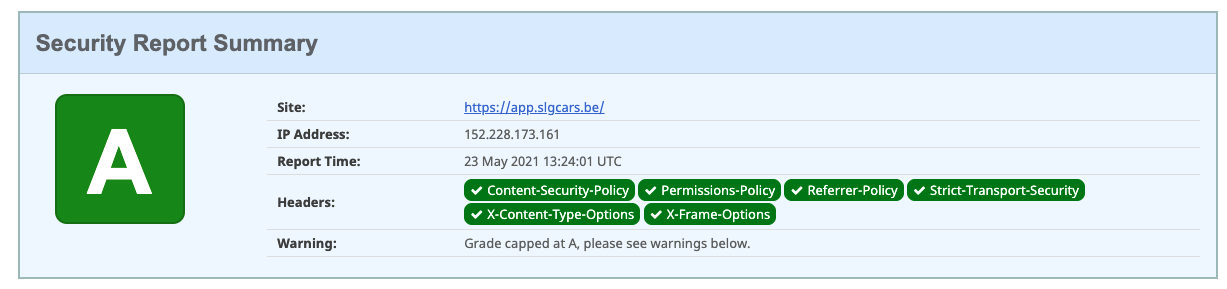
\includegraphics[width=\linewidth]{img/securityHeaders.png}
  \caption{Résultat analyse de sécurité des headers fait sur \url{https://securityheaders.com/}}
  \label{Headers}
\end{figure}

\newpage 

\subsection{Dependabot Github}

Durant le développement de l'application, afin de ne pas réinventer la roue, il est fréquent d'utiliser des packages/composants externes créés par d'autres développeurs. Ces packages étant utilisés par un grand nombre d'utilisateurs, ils sont une proie "facile" pour des personnes malveillantes qui souhaiteraient infecter un grand nombre de site-web. Ces packages sont dès lors régulièrement mis à jour par les créateur afin de garantir une sécurité maximale. 

\newpara 

Mais comment savoir quand une nouvelle version d'un packages est disponible pour des raison de sécurité? Heureusement, Github propose plusieurs services permettant de réaliser des analyse de sécurité statique sur le code y étant hébergé. Ainsi j'ai utilisé "Dependabot" qui scan périodiquement l'ensemble des dépendances du projet afin d'y déceler de potentielles failles. Si celui-ci en trouve, il m'envoie un email me prévenant de la nature de la faille et de sa dangerosité. Il ne me reste alors plus qu'a mettre à jour le(s) package(s) concerné(s) manuellement ou d'accepter une pull-request\footnote{Demande de modification du code source par une tierce personne. Pour plus d'information, voir: \url{https://www.atlassian.com/git/tutorials/making-a-pull-request}} générée par "Dependabot".

\newpara

\begin{figure}[H]
  \centering
  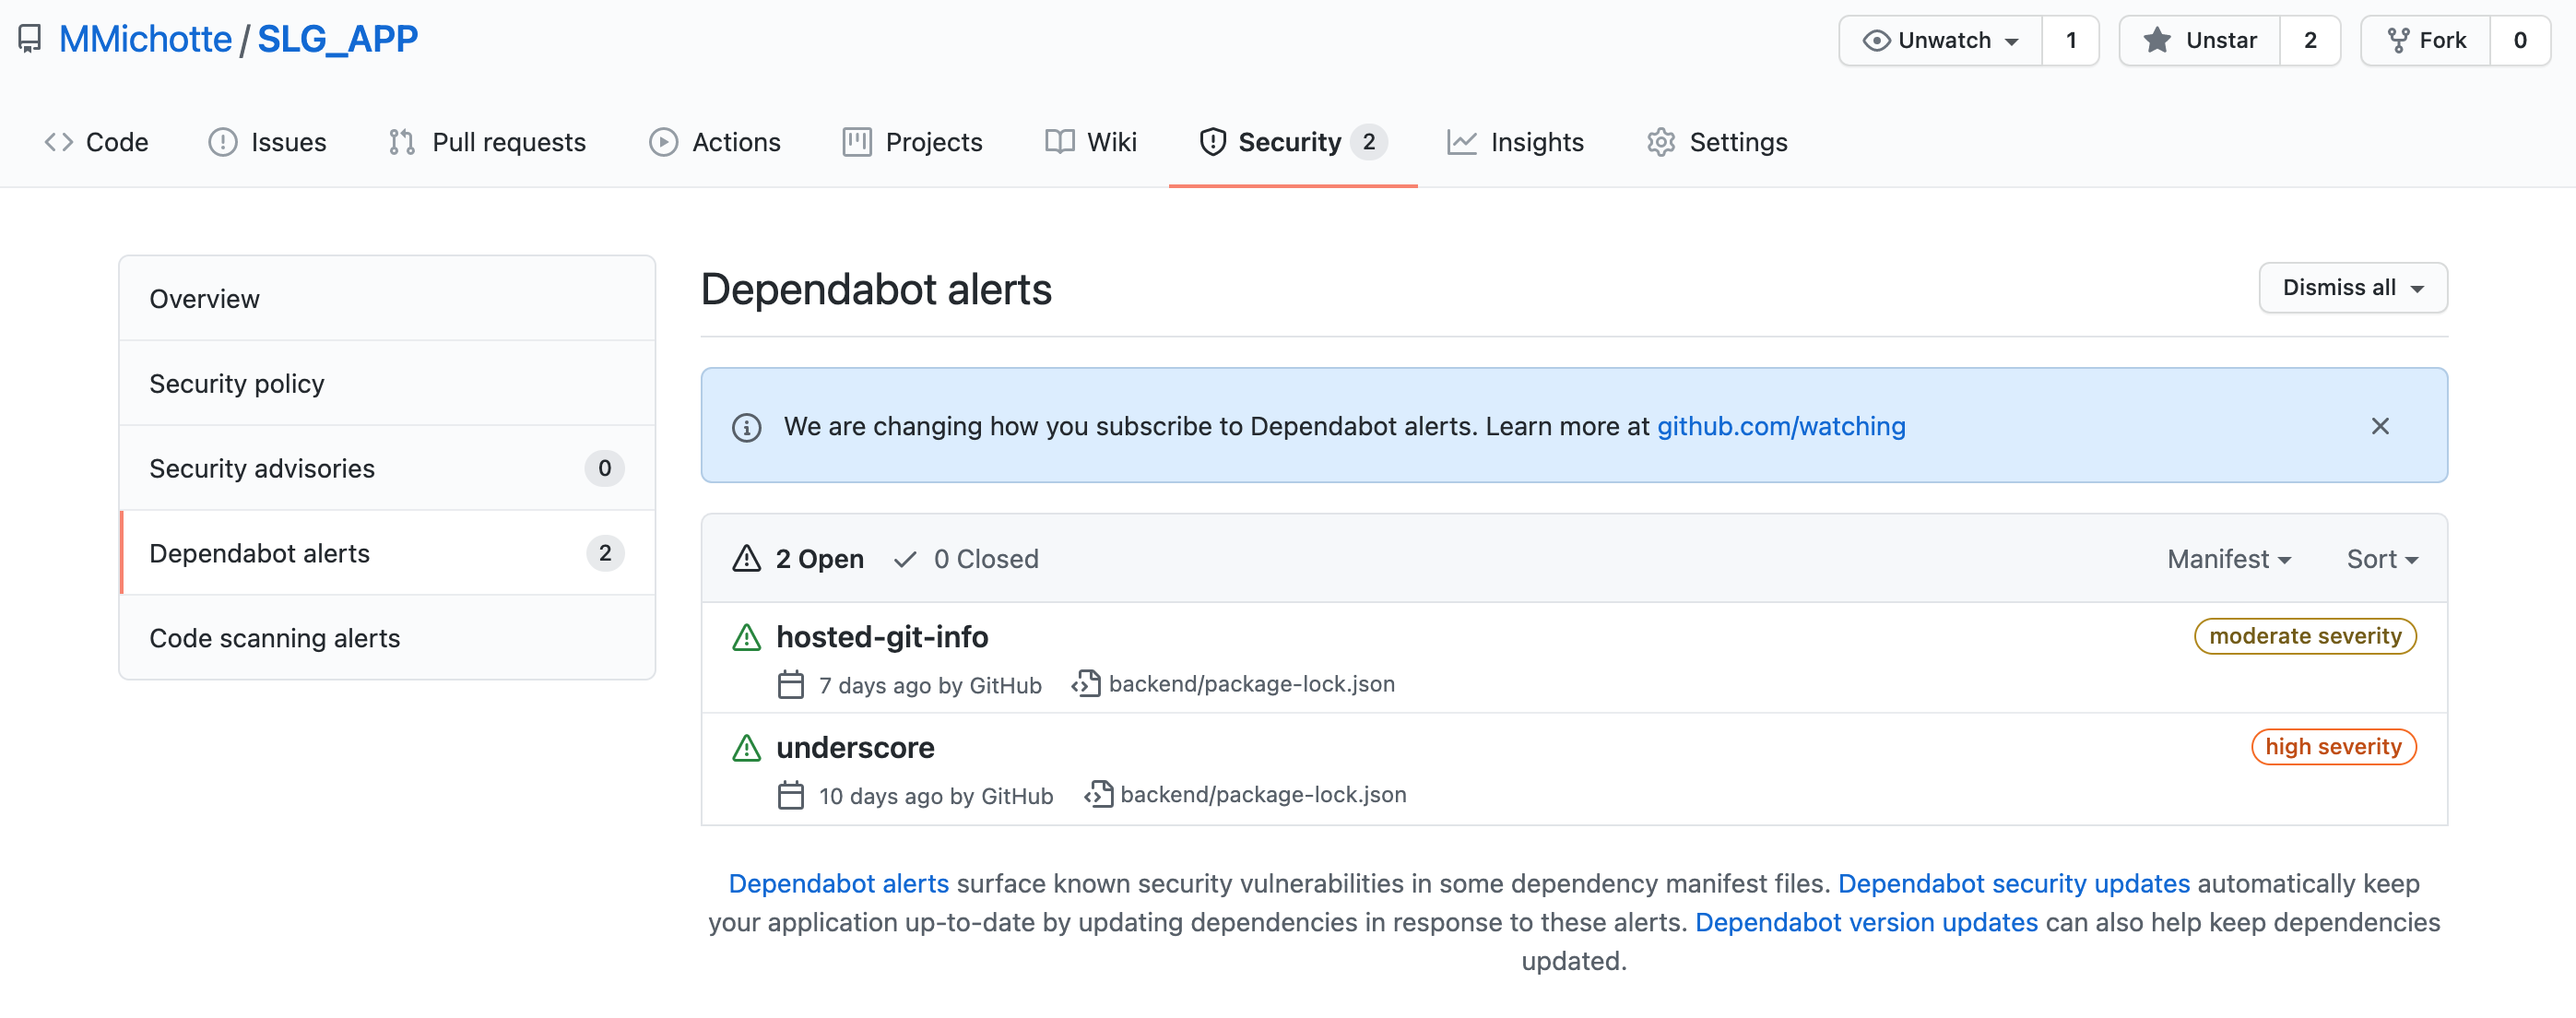
\includegraphics[width=\linewidth]{img/dependabot.png}
  \caption{Exemple d'alertes générées par "Dependabot"}
\end{figure}

\newpage
\section{Déploiement}
\subsection{Étude de marché}
\subsubsection{Avant-propos}
Il existe de nos jours une multitude de solutions afin d'héberger une application web. Toutes les solutions offrent divers avantages et inconvénients, aussi bien d'un point de vue technologique que financier. Afin de ne pas s'encombrer avec une quantité importante de possibilités, j'ai sélectionné 3 options qui me paraissent les plus adéquates :
\begin{itemize}
  \item Serveur local
  \item Heroku (\textit{\url{https://www.heroku.com/home}})
  \item Microsoft Azure (\textit{\url{https://azure.microsoft.com/en-us/}})
  \item Virtual Private Server (VPS) chez OVH (\textit{\url{https://www.ovhcloud.com/fr/vps/}})
\end{itemize}

\newpara

Dans le cadre de ce projet, il est important de préciser les points suivant :
\begin{itemize}
  \item le client n'a \textbf{pas d'informaticien} à temps pleins
  \item le client souhaite \textbf{limiter les dépenses} au maximum
  \item le \textbf{traffic} vers l'application sera \textbf{faible} car utilisé uniquement par une ou deux personnes et pendant 2-3h par jour maximum
  \item dans le futur, un web-shop pourrait être intégré à l'application et donc générer un traffic plus important -> \textbf{évolutivité}
\end{itemize}

\newpara

La solution doit pouvoir :
\begin{itemize}
  \item Héberger une application NodeJs
  \item Héberger une base de données SQL
\end{itemize}
(Idéalement les deux services sont hébergé sur la même plateforme mais ce n'est pas obligatoire.)

\newpage
\subsubsection{Étude des solutions}
\subsubsubsection{Serveur Local} 

\textbf{Déscription}: \\ Le client utilise actuellement un serveur tournant sous Windows 10 pro. Ce serveur fait tourner leur programme de gestion mais sert également d'ordinateur "classique" pour tous les employés. Notons qu'aucun système de backup automatique n'est mis en place. La base de données inclue dans leur programme de gestion devant être accessible depuis le site de la carrosserie, une règle de port-forwarding est mise en place dans le firewall de leur routeur.

\newpara
\textbf{Avantages}:
\begin{itemize}
  \item Coût négligeable car infrastructure existante
  \item Maîtrise totale des données
\end{itemize}

\newpara
\textbf{Inconvénients}:
\begin{itemize}
  \item Os du serveur inadapté (Windows 10 pro)
  \item Maintenance plus compliqué à mettre en place
  \item Scalability (évolutivité) compliquée voir impossible sans investissement conséquent
  \item Déploiement continue plus complexe à mettre en place
  \item Accessibilité extérieur require plus de sécurité
  \item Nécessite la mise en place d'une meilleur gestion des backups
  \item Pas de redondance
\end{itemize}

\newpara
\textbf{Prix}: \\ L'infrastructure physique déjà existante et l'utilisation de software gratuit et open-source tel qu'Apache, PostgreSql, fail2ban,... rendraient les coûts négligeables.

\newpara
\textbf{Coût estimé en production}: ±0 €/mois

\newpara
\textbf{Conclusion} \\ Au vu des nombreux désavantages, je pense que cette solution, bien que peu coûteuse, ne soit pas envisageable.

\newpage
\subsubsubsection{Heroku}

\textbf{Déscription}: \\ Heroku est un PaaS(Platform as a Service) fortement utilisé de par sa simplicité et sa compatibilité avec des languages modernes tel que Node, Ruby, Python et bien d'autres.
\newpara
Bien que souvent utilisé pour des projets de petite à moyenne taille, certaines grandes entreprises comme Toyota Europe ou Dubsmash l'utilisent également.

\newpara
\textbf{Avantages}:
\begin{itemize}
  \item Intégration très facile avec git
  \item Entièrement gratuite pour le développement
  \item Inclus une base de données PostgreSql
  \item Coût en production fixe
  \item Maintenance facile et accessible à distance
  \item Portabilité élevée: il est très facile d'arrêter le service de de migré vers une autre solution. Le code n'est pas lié à Heroku
  \item Expérience: j'ai déjà plusieurs fois eu l'occasion de travailler avec Heroku, je connais assez bien la plateforme et la façon de travailler avec
  \item Métrics inclus
  \item Sécurité  
\end{itemize}

\newpara
\textbf{Inconvénients}:
\begin{itemize}
  \item Scalabilité moyenne car il faut changer de plan tarifaire en fonction du traffic
  \item Gestion de la base de données moins facile (pas de rôle différents)
  \item Cold-starts d'une à deux minutes du site-web (uniquement avec la version gratuite)
\end{itemize}

\newpara
\textbf{Prix}: \\ Heroku fonctionne sur base de plans tarifaire prédéfini mais modulable. En fonction des besoins du client, j'ai sélectionné 4 plans tarifaire:
\begin{itemize}
  \newpage
  \item \textbf{Hobby - gratuit}: \\ Ce plan tarifaire offre pratiquement toutes les fonctionnalités dont nous avons besoin. Nous serons néanmoins restraint par le nombre de requêtes, la taille de la base de données, les cold-starts, ... Cette solution me semble plus que suffisante durant le développement de l'application et pourquoi pas durant les premièrs mois ou premières années d'utilisation. Attention, la DB gratuite est limitée à 10K lignes.
  \begin{figure}[H]
    \centering
    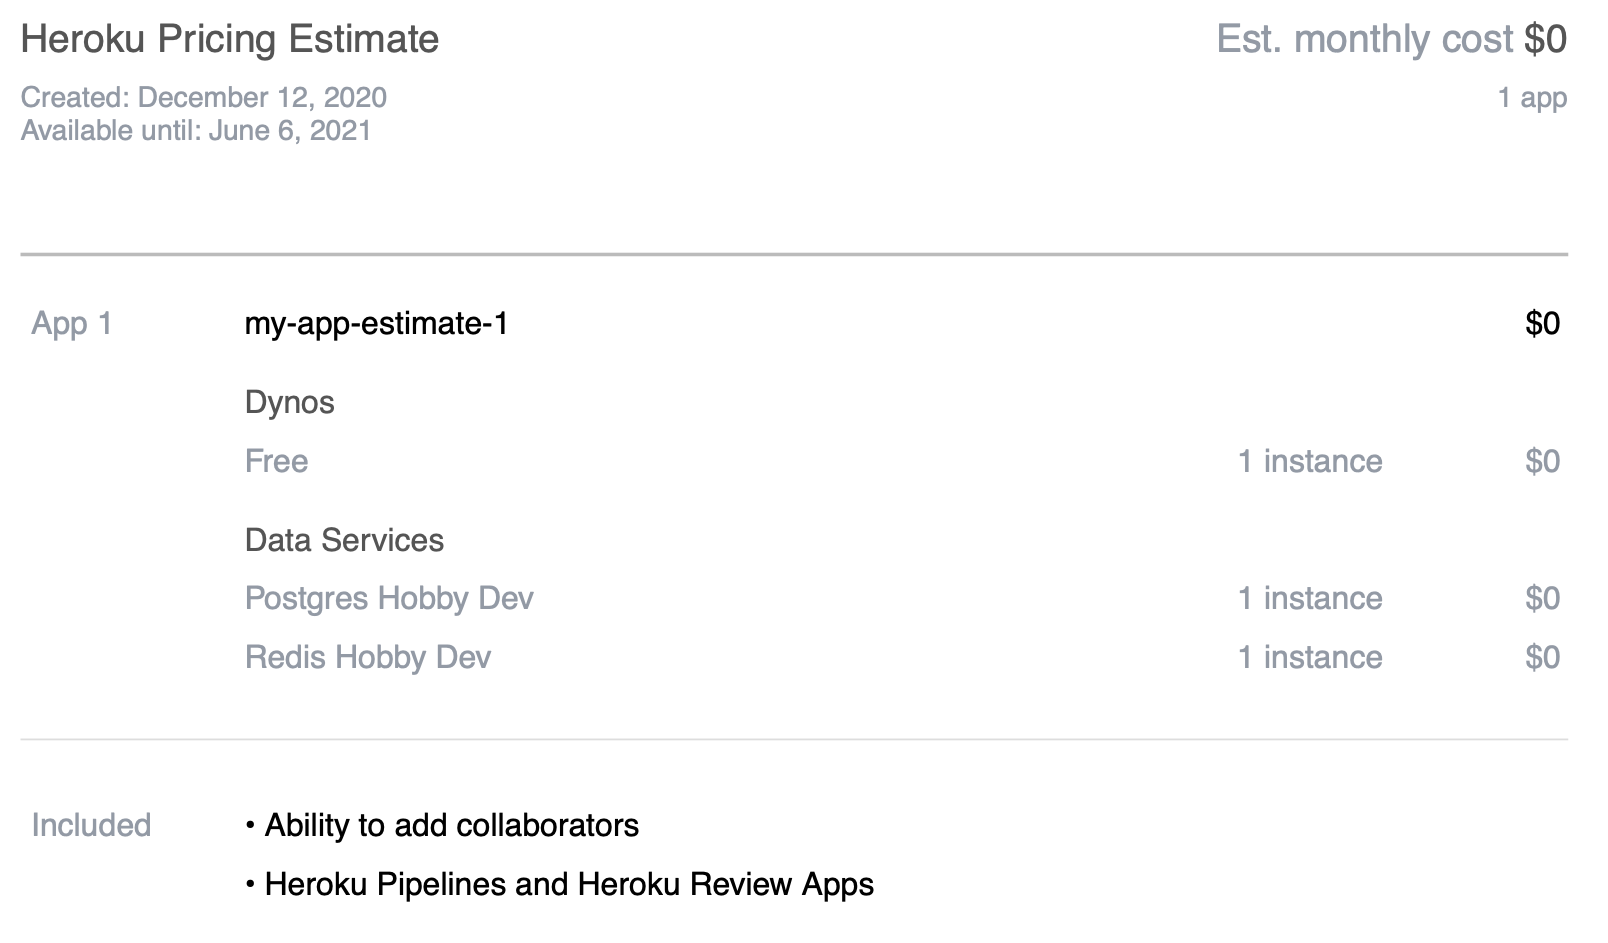
\includegraphics[width=0.75\linewidth]{img/heroku/Heroku_free.png}
  \end{figure}

  \item \textbf{Hobby - basic}: \\ Ce plan tarifaire est identique au précédent sauf que la DB peut accueillir 10M de lignes.
  \begin{figure}[H]
    \centering
    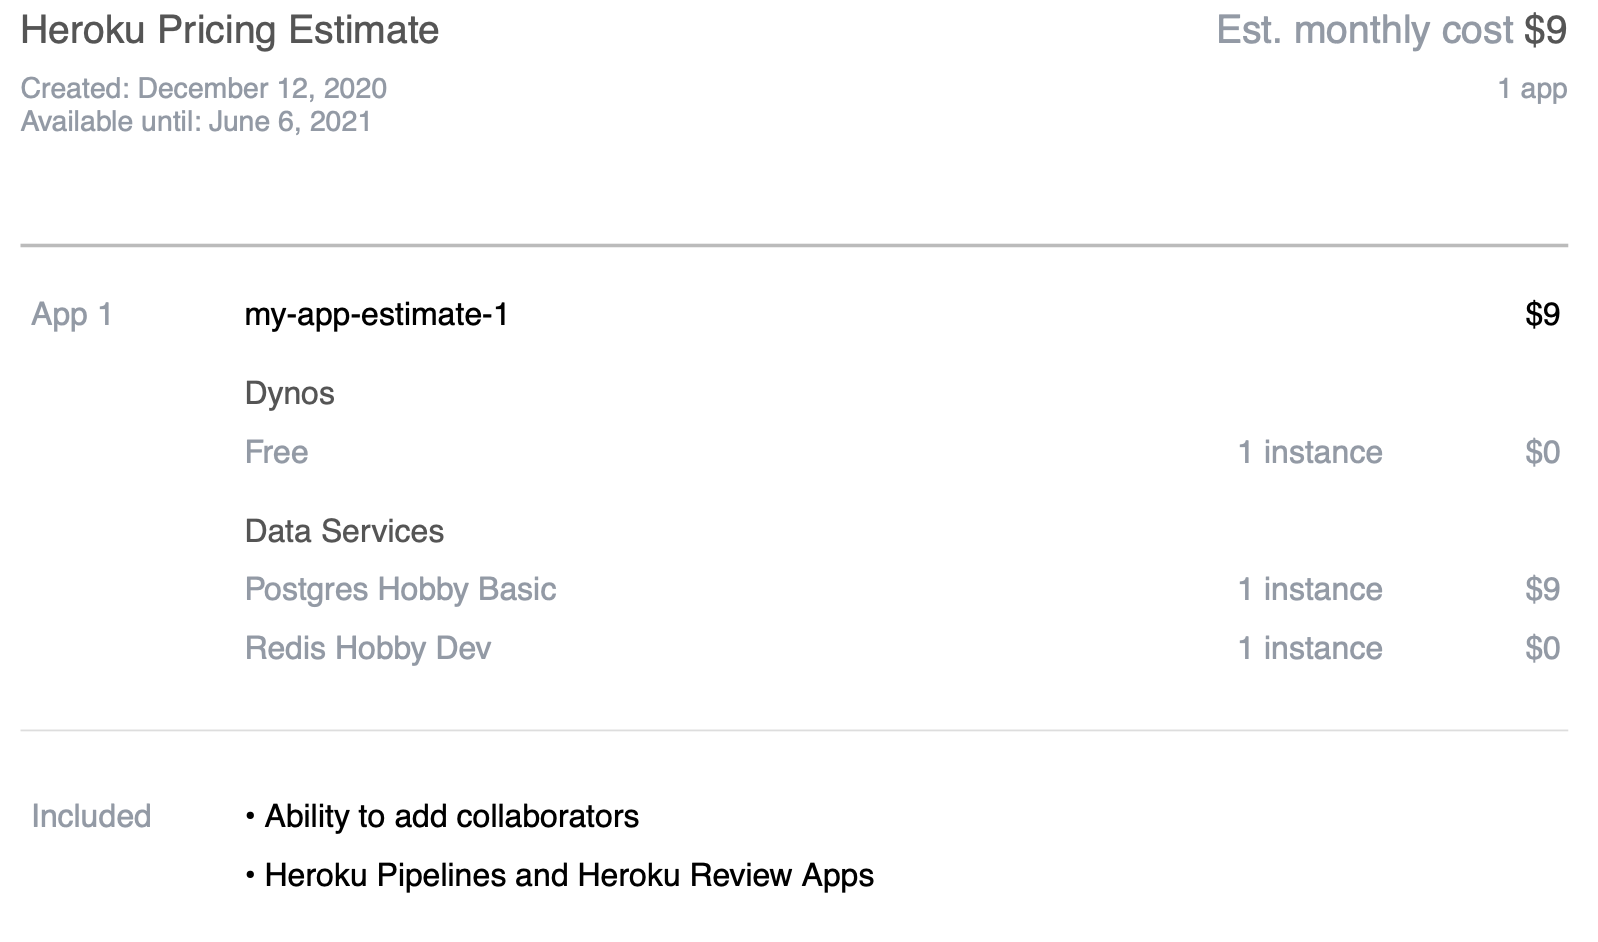
\includegraphics[width=0.75\linewidth]{img/heroku/Heroku_basic.png}
  \end{figure}
  
  \newpage
  \item \textbf{Hobby - avancé}: \\ Ce plan tarifaire est à peu de choses prêt équivalent au plan gratuit. Il permet néanmoins de supprimer complètements les cold-starts. Il offre également un les métriques du site pour les dernières 24h.
  \begin{figure}[H]
    \centering
    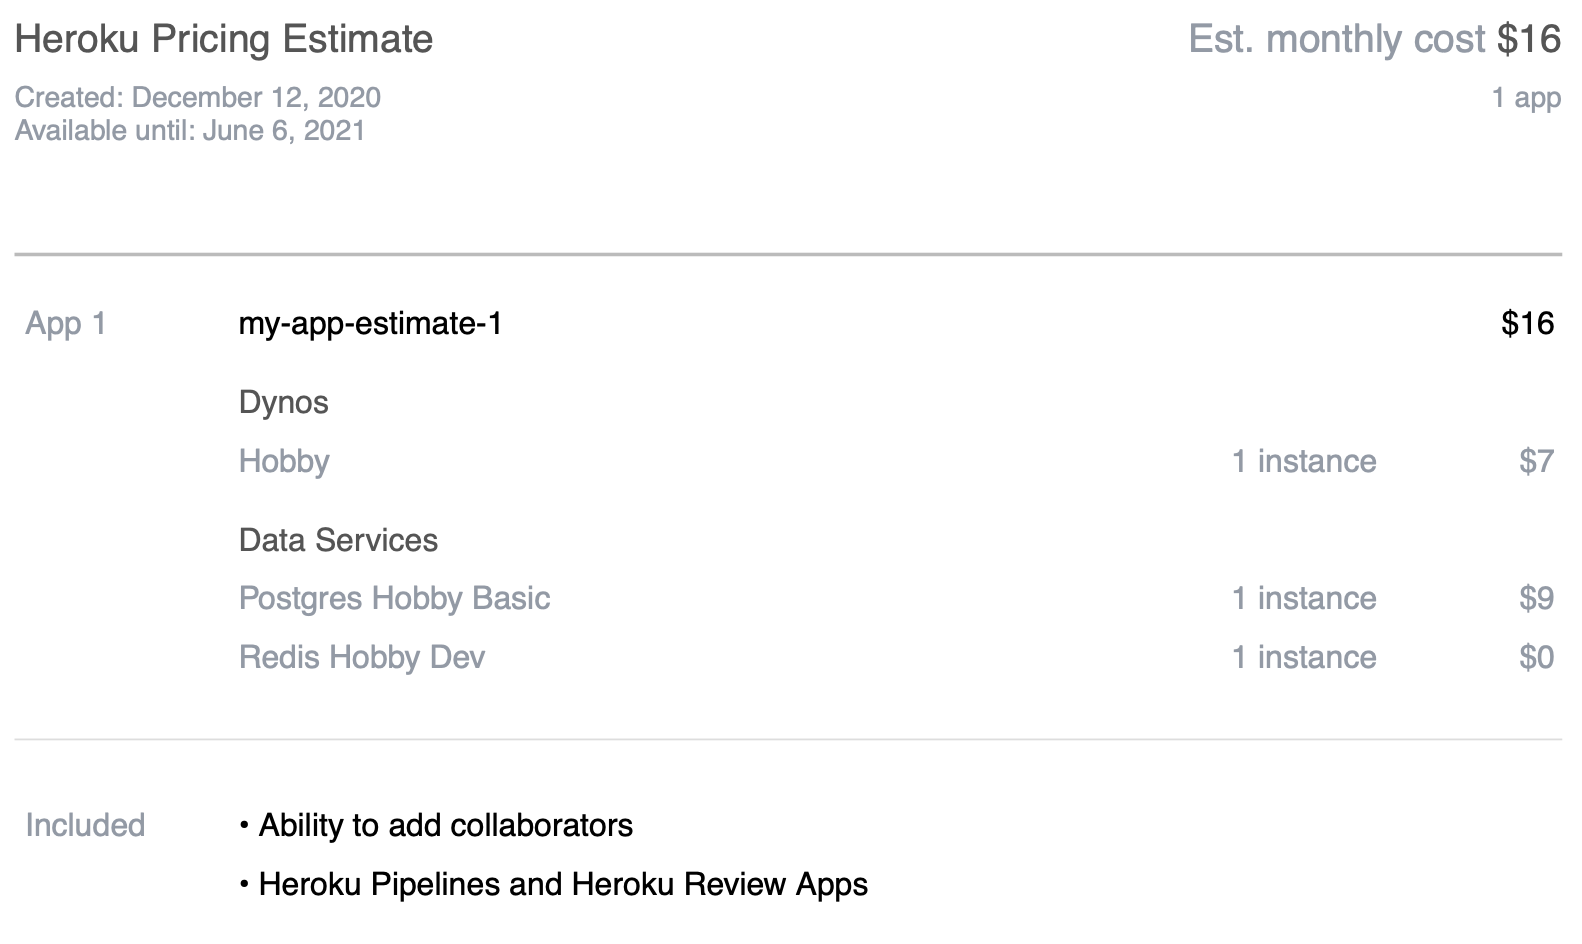
\includegraphics[width=0.75\linewidth]{img/heroku/Heroku_hobby.png}
  \end{figure}
  
  \item \textbf{Production}: \\ Cet plan offre tout ce que les plans précédents offraient mais augmente considérablement les capacité de gestion de traffic, augmente la taille maximale de la base de données, offre des métriques détaillées aussi bien pour la base de données que pour le site-web, permet des roll-backs sur une période de 7 jours.
  \begin{figure}[H]
    \centering
    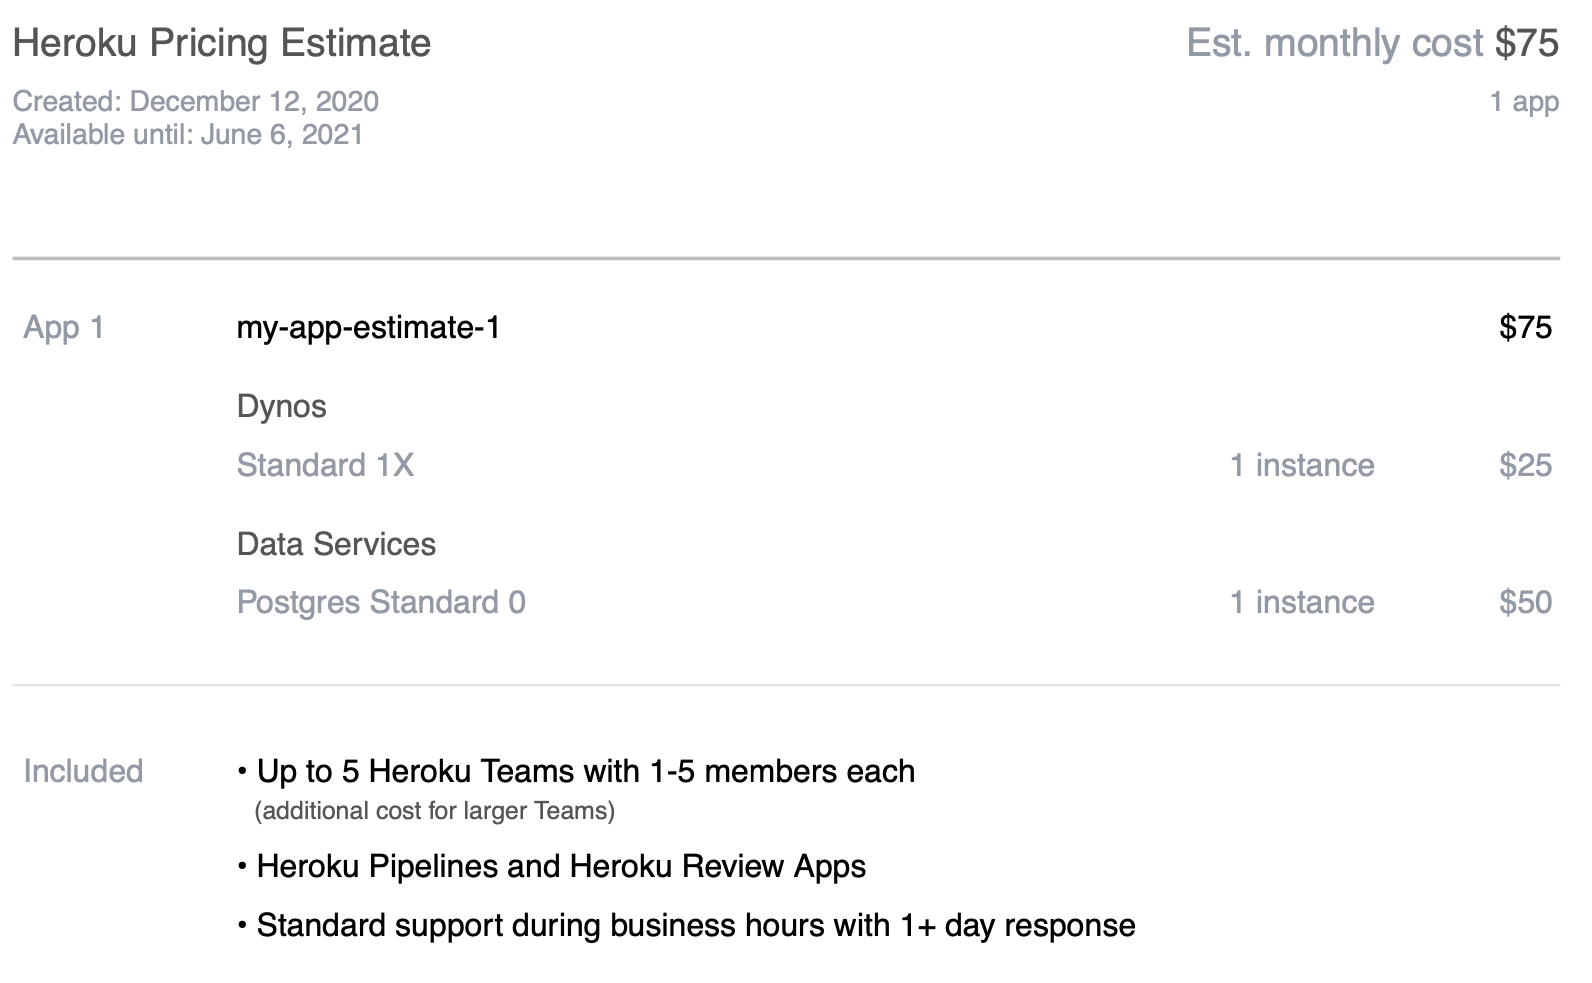
\includegraphics[width=0.75\linewidth]{img/heroku/Heroku_prod.png}
  \end{figure}
\end{itemize}

\newpage
\textbf{Conclusion} \\ Sur base de ces options, je pense qu'il est possible de partir dans un premier temps sur le plan tarifaire n°2. Néanmoins le jour où un web-shop est ajouté à l'application, il faudra probablement passer sur un autre plan tarifaire tel que le n°3.
\newpara
En plus du coût du plan n°2, il est bon de prendre une petite marge de sécurité afin de ne pas être surpris lors d'éventuels coûts supplémentaires tel qu'un nom de domaine, un autre certificat SSL,...

\newpara
\textbf{Coût estimé en production}: 18 €/mois

\newpage
\subsubsubsection{Microsoft Azure}

\textbf{Déscription}: \\ Microsoft Azure est un des leaders dans le domaine des cloud service providers. La plateforme offre plus de 200 produits couvrant une multitudes de domaines allant de la location de resources de calculs pour du Machine Learaning à l'hébergement de base de données en passant par la gestions de conteneurs Docker.
\newpara
Microsoft Azure est utilisé par un très grands nombre d'entreprises tel que 3M, Airbus, Avid, BMW et bien d'autres.

\newpara
\textbf{Avantages}:
\begin{itemize}
  \item Scalabilité extrêmement performante
  \item Compartimentation de chaque service
  \item Documentation et communauté très active
  \item Grandes flexibilité de configuration
  \item Maintenance facile et accessible à distance
  \item Métrics inclus
  \item Sécurité
\end{itemize}

\newpara
\textbf{Inconvénients}:
\begin{itemize}
  \item Coût très variable et difficile à prévoir à l'avance
  \item Complexe à configurer correctement
  \item Plus de choses à configurer manuellement
  \item Je n'ai aucune expérience
\end{itemize}

\newpara
\textbf{Prix}: \\ A l'inverse de Heroku, Azure ne fonctionne pas sur base de plans tarifaire spécifique mais fonctionne sur base du principe Pay-as-you-go. Le coût dépend donc fortement du traffic, de la taille de la base de données, de la taille des requêtes etc.

\begin{itemize}
  \item \textbf{Service Web}: Hébergement de l'app sur une machine Linux :
  \begin{itemize}
    \item version gratuite pendant 12 mois
    \item version payante : 11.081€/mois
  \end{itemize}
  \item \textbf{Base de donnée}:
  \begin{itemize}
    \item 5GB (5GB étant le minimum configurable) d'espace de stockage à 0.1155€/GB/mois soit : ±5.8€/mois
    \item 1 vCore à 0.4840€/heure, si utilisation 2h/j -> 60h/mois soit : ±29€/mois
  \end{itemize}
\end{itemize}

\newpara
\textbf{Coût estimé en production}: 50 €/mois

\newpara
\textbf{Conclusion} \\ Bien que Microsoft Azure offre une très grande flexibilité et environnement très professionnel, le coût semble fort élevé et pas très compétitif pour une application de cette envergure. Néanmoins, le jour où un web-store est ajouté, cette solution peut être retenue!

\newpage
\subsubsubsection{VPS OVH}

\textbf{Déscription}: \\ Qu'est ce qu'un VPS? \textit{"Un serveur privé virtuel est un environnement isolé, créé sur un serveur physique à partir d’une technologie de virtualisation. Cette solution offre tous les avantages d’un serveur standard, profitant de ressources allouées et d’une administration complète."}\cite{VPS}

\newpara
Il existe plusieurs entreprises de Cloud Computing offrant des services VPS tel que AWS, IBM et OVH. Ayant eu de bons échos d'OVH et ayant déjà travaillé avec leurs services, j'ai choisi de limiter ma recherche d'offre à OVH.

\newpara
\textbf{Avantages}:
\begin{itemize}
  \item Maîtrise totale des données
  \item Facile à mettre en place
  \item Grandes flexibilité de configuration
  \item Maintenance facile et accessible à distance
  \item Scalability (évolutivité) compliquée 
  \item Métrics inclus
\end{itemize}
  
\newpara
\textbf{Inconvénients}:
\begin{itemize}
  \item Nécessite la mise en place de la sécurité du VPS
  \item Nécessite la mise en place d'une gestion des backups
  \item Redondance plus compliqué à mettre en place
\end{itemize}

\newpara
\textbf{Prix}: \\ OVH propose une multitude de plans tarifaires pour leurs VPS (voir \textit{figure \ref{ovh-pricing}} ci-dessous). Notre application étant réservé à un usage interne, le traffic généré sera faible. Le plan tarifaire le moins cher nous sera dès lors plus que suffisant. De plus il est toujours possible de changer de plan par la suite. 
\begin{figure}[H]
  \centering
  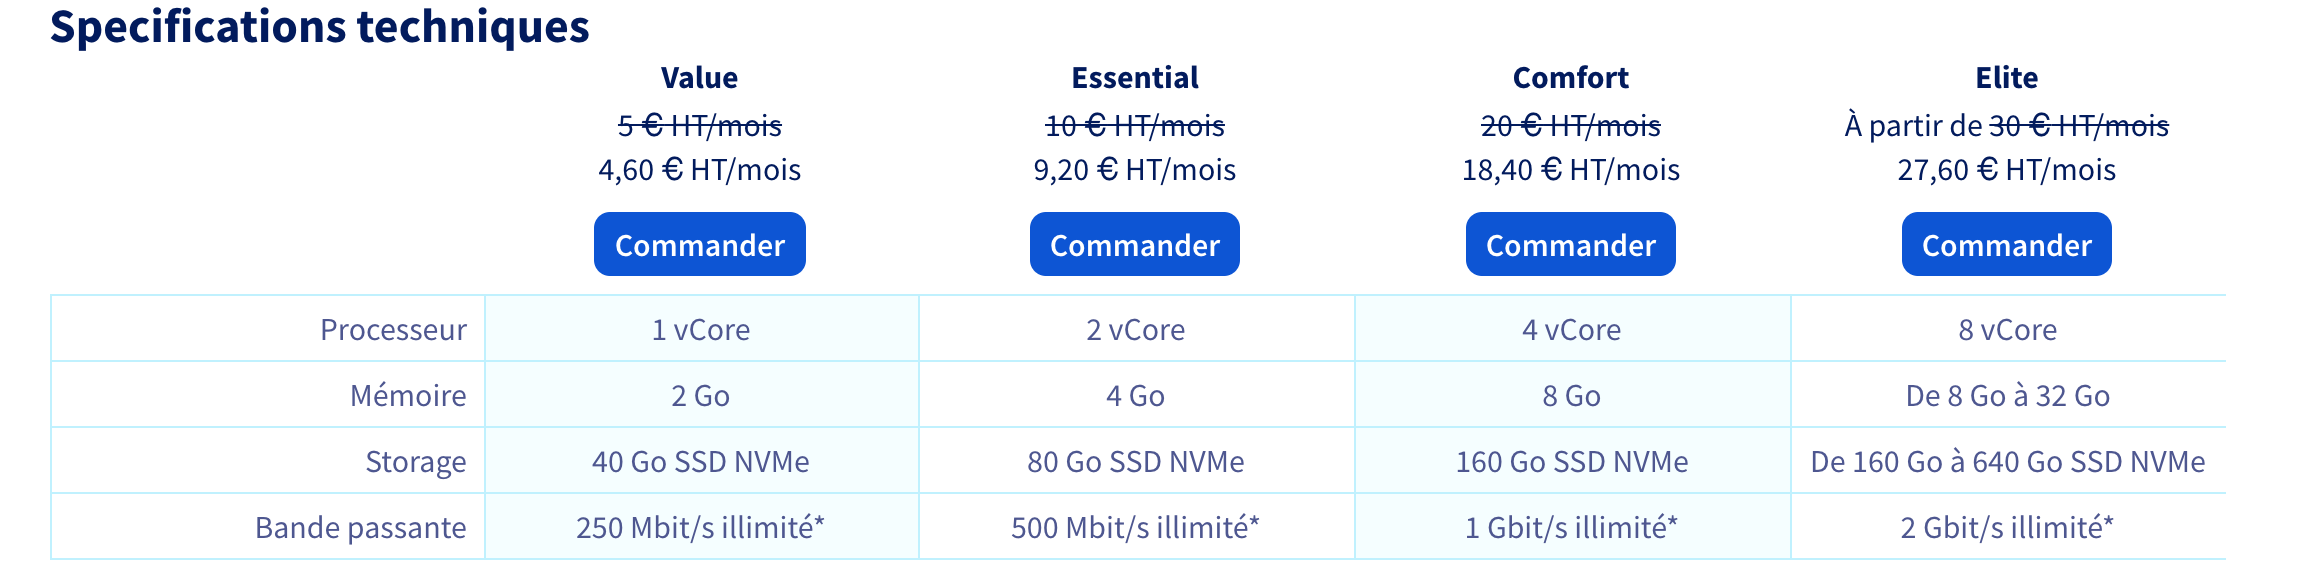
\includegraphics[width=\linewidth]{img/vps-tarifs.png}
  \caption{Tarifs VPS OVH}
  \label{ovh-pricing}
\end{figure}



\newpara
\textbf{Coût estimé en production}: ±5 €/mois

\newpara
\textbf{Conclusion} \\ Cette solution offre pratiquement tous les avantages d'un serveur local sans devoir se soucier de l'aspect hardware et ce à un prix très raisonnable. 

\newpage
\subsection{Première approche - Heroku}
Dans un but de réduire au maximum les coûts et de simplifier les choses durant le développement de l'application, le client et moi même avons décidé de déployer, dans un premier temps, celle-ci sur Heroku avec le plan gratuit. Cette solution fut plus que suffisante pendant les deux trois premiers mois du développement. Néanmoins, une fois l'application plus complète, plusieurs facteurs tel que: 
\begin{itemize}
  \item la lenteur de mise en production (temps nécessaire entre l'action de déploiement et l'accessibilité du site)
  \item le maximum de 10k lignes d'entrées dans la base de donnée 
\end{itemize}
nous ont fait revoir les solutions de déploiement. 

\subsection{Seconde approche - VPS}
Pour les raisons précédemment abordées, nous avons décidé de migré l'application hébergée sur Heroku vers un VPS chez OVH. Ceci nous a permis de nous affranchir totalement des contraintes liés à la base de données mais impliquait une plus grande configuration initiale. 

\newpara

En sachant que l'application pouvait potentiellement encore être migrée dans le future, j'ai décidé de mettre en place une multitudes d'élements afin de rendre ces transitions les plus simples possible. Ainsi l'entièreté de l'application est conteneurisée\footnote{\textit{"La conteneurisation informatique permet de packager tous les services, scripts, API, librairies dont une application a besoin. L’objectif : en permettre l’exécution sur n’importe quel noyau compatible."}\cite{conteneurisation}} et toutes les configurations du VPS sont au maximum scriptées. 

\subsubsection{Dockerisation}
Dans le but de faciliter la configuration des différents services nécessaires au bon fonctionnement de l'application, je les ai chacun mis dans un conteneur docker. Ainsi l'application est composée de 3 conteneurs distincts: 

\newpara

\begin{enumerate}
  \item \textbf{slg-db}: La base de donnée PostgreSql. Port exposé: \textbf{5434}.
  \item \textbf{slg-app}: L'application NodeJs\footnote{NodeJs est un environnement d'exécution open-srouce et multi-platforme permettant de faire tourner du code Javascript.} en tant que tel, composée du backend et frontend. Port exposé \textbf{8080}. 
  \item \textbf{caddy}: Serveur web Caddy\footnote{\url{https://caddyserver.com}} utilisé en tant que reverse-proxy\footnote{Un reverse-proxy est un intermédiaire de communication réseau permettant de transmettre une requête au serveur cible en fonction du nom de domaine de cette requête.} et gestionnaire des certificats https. Ports exposés: \textbf{80} et \textbf{441}.
\end{enumerate}

\newpage

Ces trois conteneurs fonctionnent en symbiose et sont dépendant les un des autres. L'application node ne démarrera par exemple pas si la base de donnée n'a pas démarrée avec succès. Afin de controller l'environnement dans lesquels ces conteneurs sont lancés ainsi que de pouvoir facilement les démarrer/arrêter, j'ai créé un fichier docker-compose\footnote{docker-compose permet d'orchestrer un ensemble de conteneurs dans le but de simplifier la gestion et la communication de ceux-ci.}. \\ (Voir: \url{https://github.com/MMichotte/SLG_APP/blob/master/docker/docker-compose.yml})

\subsubsection{Scirpts}
J'ai principalement écrit 2 scripts, le premier et plus consistent me permet de configurer automatiquement un nouveau VPS. Dans les faits, celui ci exécute: 
\begin{enumerate}
  \item Mise à jour des packages
  \item Mise à jour de la time-zone
  \item Création d'un nouvel utilisateur
  \item Modification des paramètres de connexion SSH
  \item Configuration et activation de Fail2ban\footnote{Fail2ban est un programme de prévention permettant de bloquer les tentatives d'intrusion frauduleuses}
  \item Installation de docker-compose
\end{enumerate}

\newpara

Le second script est bien moins complexe et me permet de configurer et démarrer le backup (local) journalier de la base de donnée. Ces backups sont réalisé périodiquement à l'aide de crontab\footnote{\textit{"Crontab est un outil qui permet de lancer des applications de façon régulière, pratique pour un serveur pour y lancer des scripts de sauvegardes, etc."}\cite{CRON}}.

\newpara

Il s'avère que ces scripts m'ont été très rapidement utile. Seulement 6h après la configuration complète du VPS, un incendie à ravagé plusieurs data-centers chez OVH et a détruit, entre autre, notre VPS.\footnote{Plus d'information sur l'incident: \url{https://www.ovh.com/fr/news/presse/cpl1785.dernieres-informations-notre-site-strasbourg}} Après quelques jours d'inaccessibilité, j'ai pu re-configurer un VPS dans un autre data-center. Cette configuration n'a pas durée plus de 10 minutes.

\newpage

\subsubsection{Sécurité}
\subsubsubsection{SSH}
\newparasm
Une connexion SSH avec le VPS est indispensable pour pouvoir le configurer et y configurer les différents services. Cependant c'est aussi une des principales porte d'entrée pour les personnes malveillantes. Afin de minimiser au maximum les risques j'ai configuré le service ssh de tel sorte que :
\begin{itemize}
  \item il soit disponible sur le port 62222 et non 22. Un grand nombre d'attaques par force brute se basent sur le fait que par défaut le port utilisé par SSH est le 22. Dès lors changer le port par défaut permet d'éviter toute une série d'attaques automatisées. 
  \item il interdise la connexion par mote de passe. Il est désormais uniquement possible de se connecter par pair de clés SSH.
  \item il interdise la connexion en tant que root. 
\end{itemize} 

\subsubsubsection{Fail2ban}
\newparasm
Qu'est ce que Fail2ban? \textit{"fail2ban est une application qui analyse les logs de divers services (SSH, Apache, FTP…) en cherchant des correspondances entre des motifs définis dans ses filtres et les entrées des logs. Lorsqu'une correspondance est trouvée une ou plusieurs actions sont exécutées. Typiquement, fail2ban cherche des tentatives répétées de connexions infructueuses dans les fichiers journaux et procède à un bannissement en ajoutant une règle au pare-feu iptables ou nftables pour bannir l'adresse IP de la source."}\cite{F2B}

\newpara

Comme expliqué précédemment, un des points d'entrés les plus vulnérable est le service SSH. Dans le but de renforcer son imperméabilité, j'ai ajouté une règle fail2ban limitant le nombre de tentatives de connexion à 6. Après 6 connexions échouées, l'adresse IP source est bloquée pour une durée de 1h. La durée d'un ban augmente de manière exponentielle si la même IP re-tente une multitudes de connexions après s'être faite bannir. 

\newpage

\subsubsubsection{Firewall (UFW)}
\newparasm
\begin{minipage}{.5\textwidth}
  Afin de pouvoir contrôler le flux d'informations circulant entre le VPS et le réseau internet j'ai mis en place un firewall sur le VPS. Celui-ci intégrant par défaut les iptables\footnotemark, j'ai choisi d'utiliser "UFW" car celui-ci s'intègre parfaitement avec les iptables.  
\end{minipage}
\begin{minipage}{.5\textwidth}
  \begin{figure}[H]
    \centering
    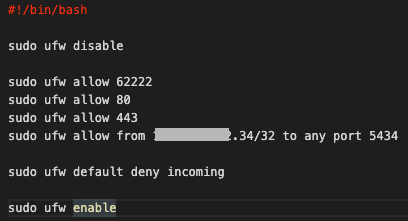
\includegraphics[width=0.8\linewidth]{img/ufw-script.png}
    \caption{Script d'ajout règles UFW}
  \end{figure}
\end{minipage}


\subsubsubsection{Firewall (OVH)}
\newparasm
En plus du firewall interne au VPS, OVH met à disposition un firewall en amont du VPS. J'ai configuré celui-ci afin d'être le plus restrictif possible (voir \textit{figure \ref{VPS-firewall}}).
\begin{figure}[H]
  \centering
  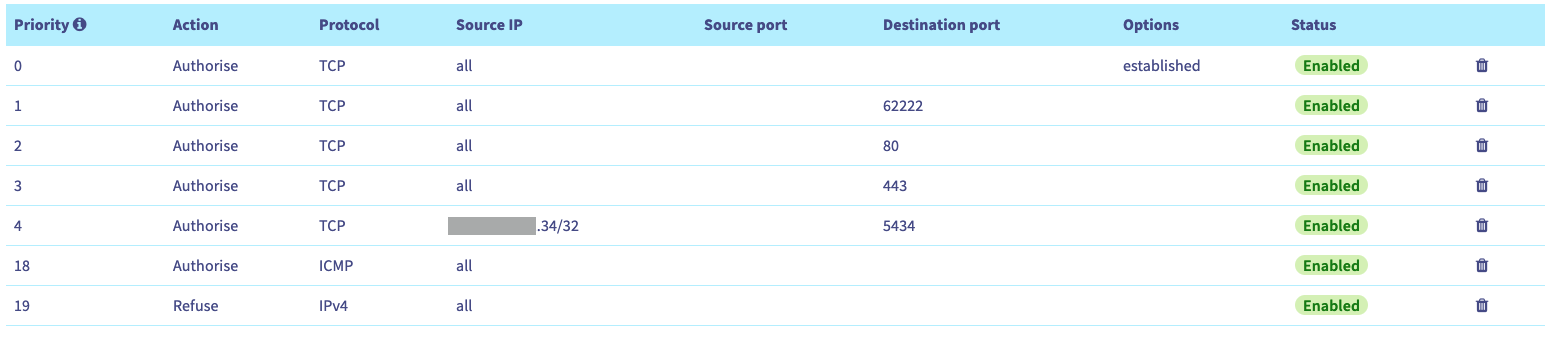
\includegraphics[width=\linewidth]{img/ovh-fireWall.png}
  \caption{Configuration du firewall en amont du VPS}
  \label{VPS-firewall}
\end{figure}

\newpara
\newpara

Notons que dans les deux firewall (UFW et OVH) le port 5434 est ouvert, ce port est utilisé par la base de donnée et rendre se port accessible publiquement est potentiellement une faille de sécurité. Néanmoins j'ai restreint l'accès à ce port à uniquement une adresse IP spécifique (la mienne en l'occurrence). Une fois l'application terminée, cette règle sera supprimée rendant la base de données totalement inaccessible depuis l'extérieur. 


\footnotetext{iptables est le pare-feu installé par défaut sur les système d'exploitation linux.}

\newpage
\subsection{Intégration et Déploiement Continu (CI/CD)}

La méthodologie Agile se basant sur une succession de "sprints" aboutissant à chaque fois à une nouvelle fonctionnalité, il est important que celle-ci puisse rapidement être testée par le client afin d'en avoir un feedback et de pouvoir y apporter ou non des modifications. 

\newpara
Dans ces conditions il est indispensable d'avoir un système d'intégration et de déploiement continu. L'intégration continue consiste à automatiser les phases de tests tandis que le déploiement continu permet d'automatiser la mise en production de la nouvelle fonctionnalité. 

\newpara
Le code de ce projet étant hébergé sur Github, j'ai pu profiter des "Github Actions"\footnote{Plus d'informations voir: \url{https://github.com/features/actions}} permettant de définir un ensemble d'actions à éxécuter sur le code et ce sur base de certaines conditions et dans un environnement isolé. pour ce projet j'ai dès lors défini le workflow suivant :
\linebreak \linebreak
Lors d'une modification du code sur la branche "master": \\
\textbf{1.} lancement en simultané des tests unitaires frontend et backend \\
Si tous les tests sont passés avec succès: \\
\textbf{2.} déploiement:
\begin{enumerate}[label=(\alph*)]
  \item Exécution d'un script bash permettant de compiler le code source
  \item Création des variables d'environnement
  \item Envoie des fichier sur le serveur 
  \item Lancement des différents services (docker-compose)
\end{enumerate}

\newpara

Exemple de résultat du CI/CD lors d'une résolution d'un bug. 
\begin{figure}[H]
  \centering
  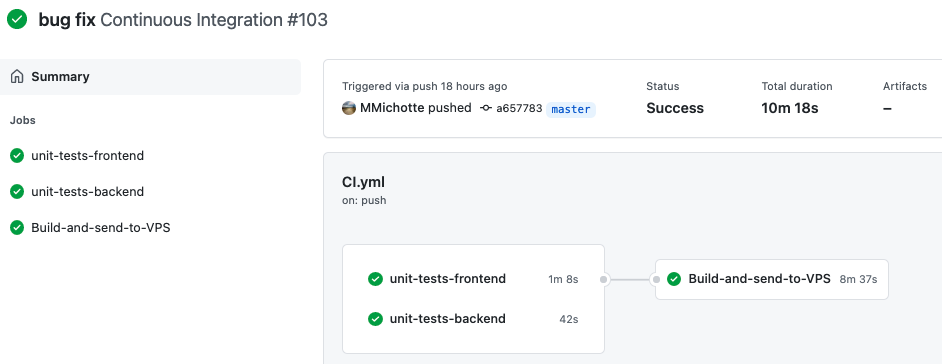
\includegraphics[width=\linewidth]{img/CI-result.png}
  \caption{Exemple résultat du CI/CD}
\end{figure}


\newpage
\section{Migration données existantes}
\subsection{Problématique}

Durant la majeur partie du développement, j'ai travaillé avec des données fictives. Une fois les fonctionnalités à "court terme" implémentées, il a fallu transférer/migrer l'ensemble des données existante du programme "Gad-Garage" vers notre nouvelle base de données. Malheureusement, le logiciel "Gad-Garage" fonctionne avec une base de données interne à celui-ci et aucun moyen n'est fourni pour pouvoir en extraire l'ensemble des données. Le logiciel permet cependant d'extraire certaines informations en format CSV\footnote{Format de fichier texte représentant des données tabulaires sous forme de valeurs séparées par un délimiteur connu, souvent une virgule.}. Néanmoins, les données contenues dans ces fichiers ne sont pas utilisable en tant que tel pour principalement deux raisons: 
\begin{enumerate}
  \item les données du CSV ne correspondent pas à la structure de la nouvelle base de données
  \item les données contiennent des informations venant de plusieurs tables différents sans en connaître la liaison.
\end{enumerate}
A titre d'exemple, le fichier contenant la commandes ne contenait pas l'identifiant d'un fournisseur mais son nom.

\subsection{Solution}

La première approche fut de contacter le service après-vente de "Gad-Garage". Après plusieurs jours d'attente et de relance, nous n'avons jamais eu de réponse. 

\newpara

Dans un second temps j'ai alors décidé de récupérer l'ensemble des fichiers sources de l'application depuis un des ordinateurs du client. Après quelques recherches j'ai trouvé les fichiers constituant la base de données mais ceux-ci étaient protégés par mot de passe. Cette solution est tombée à l'eau.

\newpara

La dernière solution fut alors de récupérer un maximum de fichiers CSV à partir de l'application elle-même et de, sur base des données qu'ils contiennent, recouper les informations afin d'en extraire les données utiles. Finalement, à l'aide de plusieurs scripts python et un travail conséquent, j'ai su récupérer approximativement 95\% des données.

\newpage
\section{Monitoring et Backups}

\subsection{Monitoring}
Afin d'être tenu au courant de l'état de l'application web, il est important de mettre en place un système de monitoring. OVH met à disposition un panneau de contrôle permettant de visualiser certaines informations propres au VPS tels que l'utilisation du CPU, de la mémoire ou encore le trafic réseau. Ces informations sont intéressantes dans le but de déterminer si les performances du VPS conviennent pour l'application mais ne permettent pas de déceler une éventuelle indisponibilité de l'application. 

\newpara

Dès lors, dans le but de connaître l'état de disponibilité de l'application, j'ai utilisé "UptimeRobot"\footnote{\url{https://uptimerobot.com}}. En plus de pouvoir consulter l'état de disponibilité sur l'application web, celle-ci peut envoyer un email d'alerte dans l'éventualité où le site serait indisponible.

\begin{figure}[H]
  \centering
  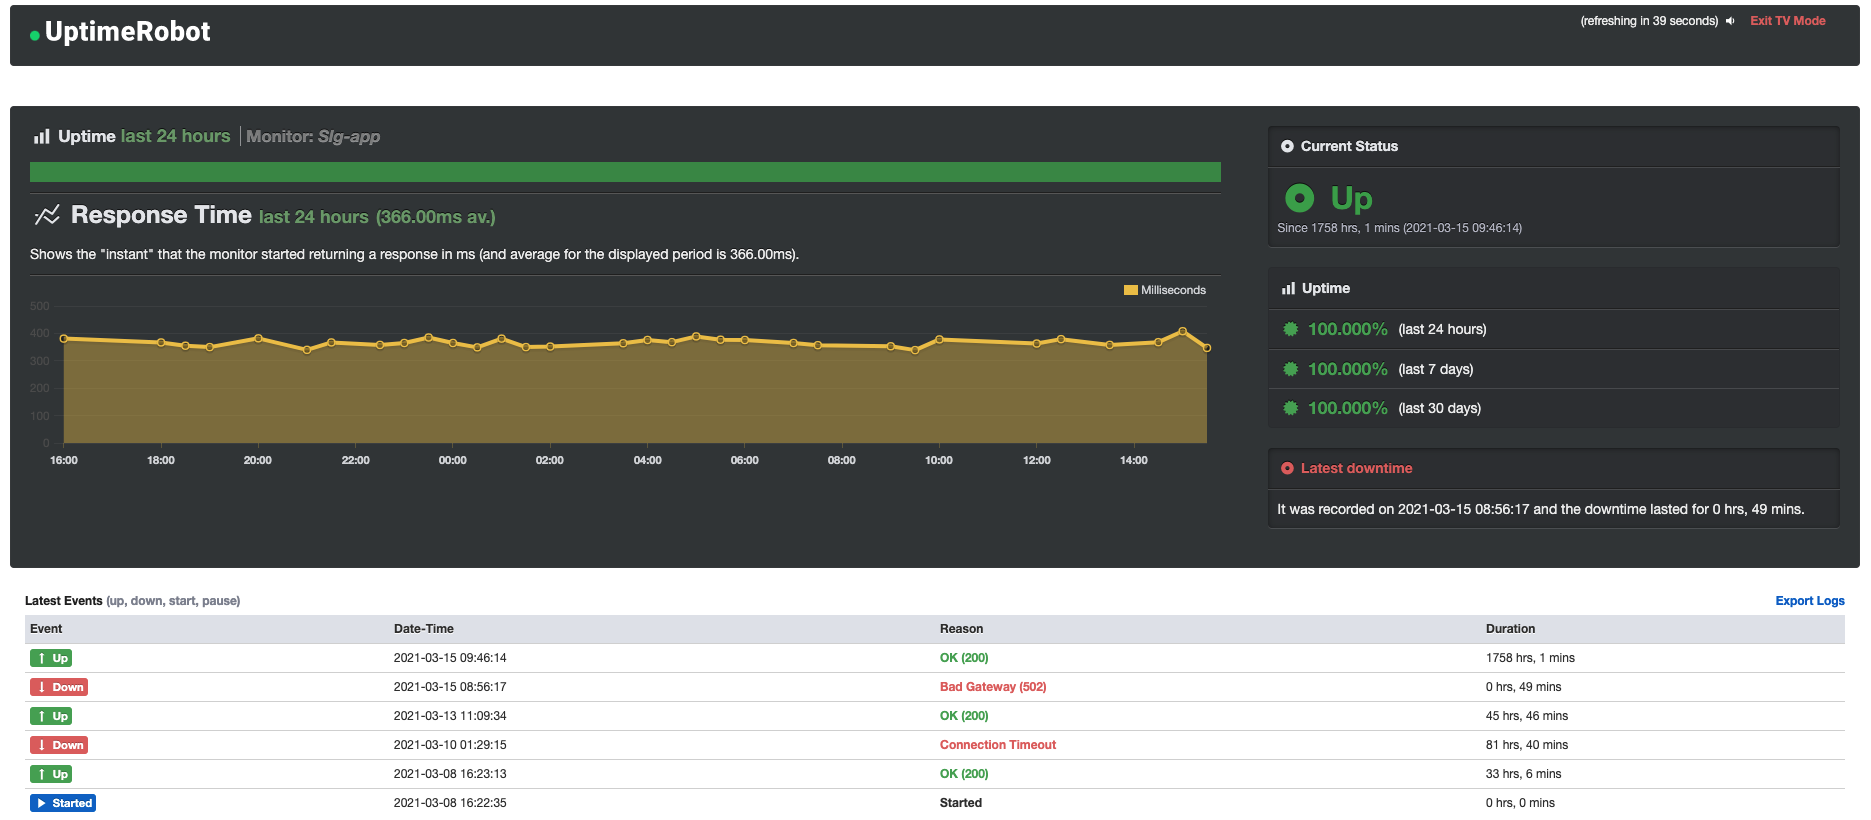
\includegraphics[width=\linewidth]{img/uptimeRobot.png}
  \caption{Dashboard monitoring de l'application - UptimeRobot}
\end{figure}

\newpara

Dans le futur il serait intéressant de mettre en place un monitoring plus approfondi permettant de récupérer des informations plus détaillées à partir des conteneurs docker. Ceci peut être obtenu à l'aide d'outils tels que "Prometheus"\footnote{\url{https://prometheus.io}} ou "Sematext"\footnote{\url{https://sematext.com/docker/}} 

\newpage

\subsection{Backups}

Comme expliqué dans la seconde partie du \textit{chapitre \ref{scritps}}, un backup de la base de données est effectué quotidiennement. Cependant ces backups sont stockés sur le VPS lui-même. En cas de perte du VPS, les backups sont eux aussi perdus.

\newpara

A terme, il faudra externaliser les backups. OVH propose une solution payante à laquelle nous souscrirons probablement une fois l'application terminée dans son intégralité.

\newpage
\section{Conclusion}

Ce travail m'a permis d'approfondir et maîtriser plusieurs aspects de la réalisation d'une application pour un client. En particulier:

\vskip 0.5cm

\textbf{1. L'analyse} \\Entre l'organisation de réunions avec le client, la traduction de ses besoins en user stories ou encore le design de la base de données, il n'était pas toujours facile de s'adapter aux demandes du client. Néanmoins, j'ai pu m'adapter et j'ai appris à combiner l'analyse et le développement de façon à être le plus productif possible. 

\vskip 0.5cm
\textbf{2. Le développement} \\Tout au long du développement, j'ai appris une grande quantité de techniques dans le but d'améliorer non seulement la qualité du code mais aussi sa robustesse et sa lisibilité. 

\vskip 0.5cm
\textbf{3. La mise en production} \\J'avais par le passé déjà utilisé des techniques de déploiement continu mais pas dans le but de réellement déployer l'application dans un milieu de production. Ceci amène une série de "challenges" qui m'ont obligé à être très rigoureux. 

\newpara

Bien que l'application ne soit pas terminée, les objectifs fixés avec le client en début de projet ont été atteints. Les fonctionnalités jusqu'à présent implémentées sont fortement appréciées par le client. Celui-ci m'a d'ailleurs demandé de continuer le travail pour délivrer une application complète. Ceci fera l'objet d'une prochaine collaboration. 

\newpara

Personnellement je suis très content d'avoir pu réaliser ce travail avec un vrai client d'autant que l'application lui sera d'une réelle utilité. Ce travail m'a permis de mettre en oeuvre les notions acquises durant ces années études et d'acquérir une réelle expérience du métier de développeur en tant que "freelance". 

\newpage
\section{Définitions}

\begin{description}
  \item[US]: User Story 
  \item[CI]: Continuous Integration 
  \item[CD]: Continuous Deployment 
  \item[IDE]: Integrated Development Environment 
  \item[API]: Application Programming Interface
\end{description}

\newpage
\section{Bibliographie}

\renewcommand{\section}[2]{}%
\begin{thebibliography}{}

\bibitem{slg-website} 
Tristan Slegers (sans date), sur le site \textit{SLG Classic Cars : La voiture ancienne. Côté passion.} Consulté le 19 mai 2021.
\\\url{https://slgcars.be}

\bibitem{SI}
Syloé (2021), sur le site \textit{syloe: Système d'information} Consulté le 20 mai 2021
\\\url{https://www.syloe.com/glossaire/systeme-dinformation/}

\bibitem{GAD}
E.U.R.L ADELIE (2021), sur le site \textit{Logiciel Garage | Logiciel Garage Professionnel , GAD Garage .} Consulté le 20 mai 2021
\\\url{https://www.logiciel-garage.fr}

\bibitem{User-Story}
Walter Görlitz (21 février 2021), sur le site \textit{User story - Wikipedia} Consulté le 22 mai 2021
\\\url{https://en.wikipedia.org/wiki/User_story}

\bibitem{Mock}
Verdy P (31 janvier 2021), sur le site \textit{Mock-up — Wikipédia} Consulté le 22 mai 2021
\\\url{https://fr.wikipedia.org/wiki/Mock-up}

\bibitem{CI-CD}
Rob Terzi (16 novembre 2018), sur le site \textit{Qu'est-ce que l'approche CI/CD ?} Consulté le 22 mai 2021
\\\url{https://www.redhat.com/fr/topics/devops/what-is-ci-cd}

\bibitem{Agile}
Shadow-M-P (14 mai 2021), sur le site \textit{Méthode agile — Wikipédia} Consulté le 23 mai 2021
\\\url{https://fr.wikipedia.org/wiki/Méthode_agile}

\bibitem{Salt}
Pautard (08 avril 2021), sur le site \textit{Salage (cryptographie) — Wikipédia} Consulté le 23 mai 2021
\\\url{https://fr.wikipedia.org/wiki/Salage_(cryptographie)}

\end{thebibliography}





\end{document}